%This is the first chapter of the dissertation

%The following command starts your chapter. If you want different titles used in your ToC and at the top of the page throughout the chapter, you can specify those values here. Since Columbia doesn't want extra information in the headers and footers, the "Top of Page Title" value won't actually appear.

\chapter[Results][Results]{Results}

This chapter presents the results of the search for squarks and gluinos in zero lepton final states.
The full signal region distributions with normalization factors $\mu_B$ derived from the background-only fits are shown.
The systematic uncertainties are discussed.
As no excess is observed, we run the model-dependent fits to set exclusion limits in the sparticle-\lsp~ plane and use the model-independent fit procedure to set model-independent upper limits on the new physics cross-sections.

\section{Signal region distributions}
\begin{figure}[tbp]
\begin{center}
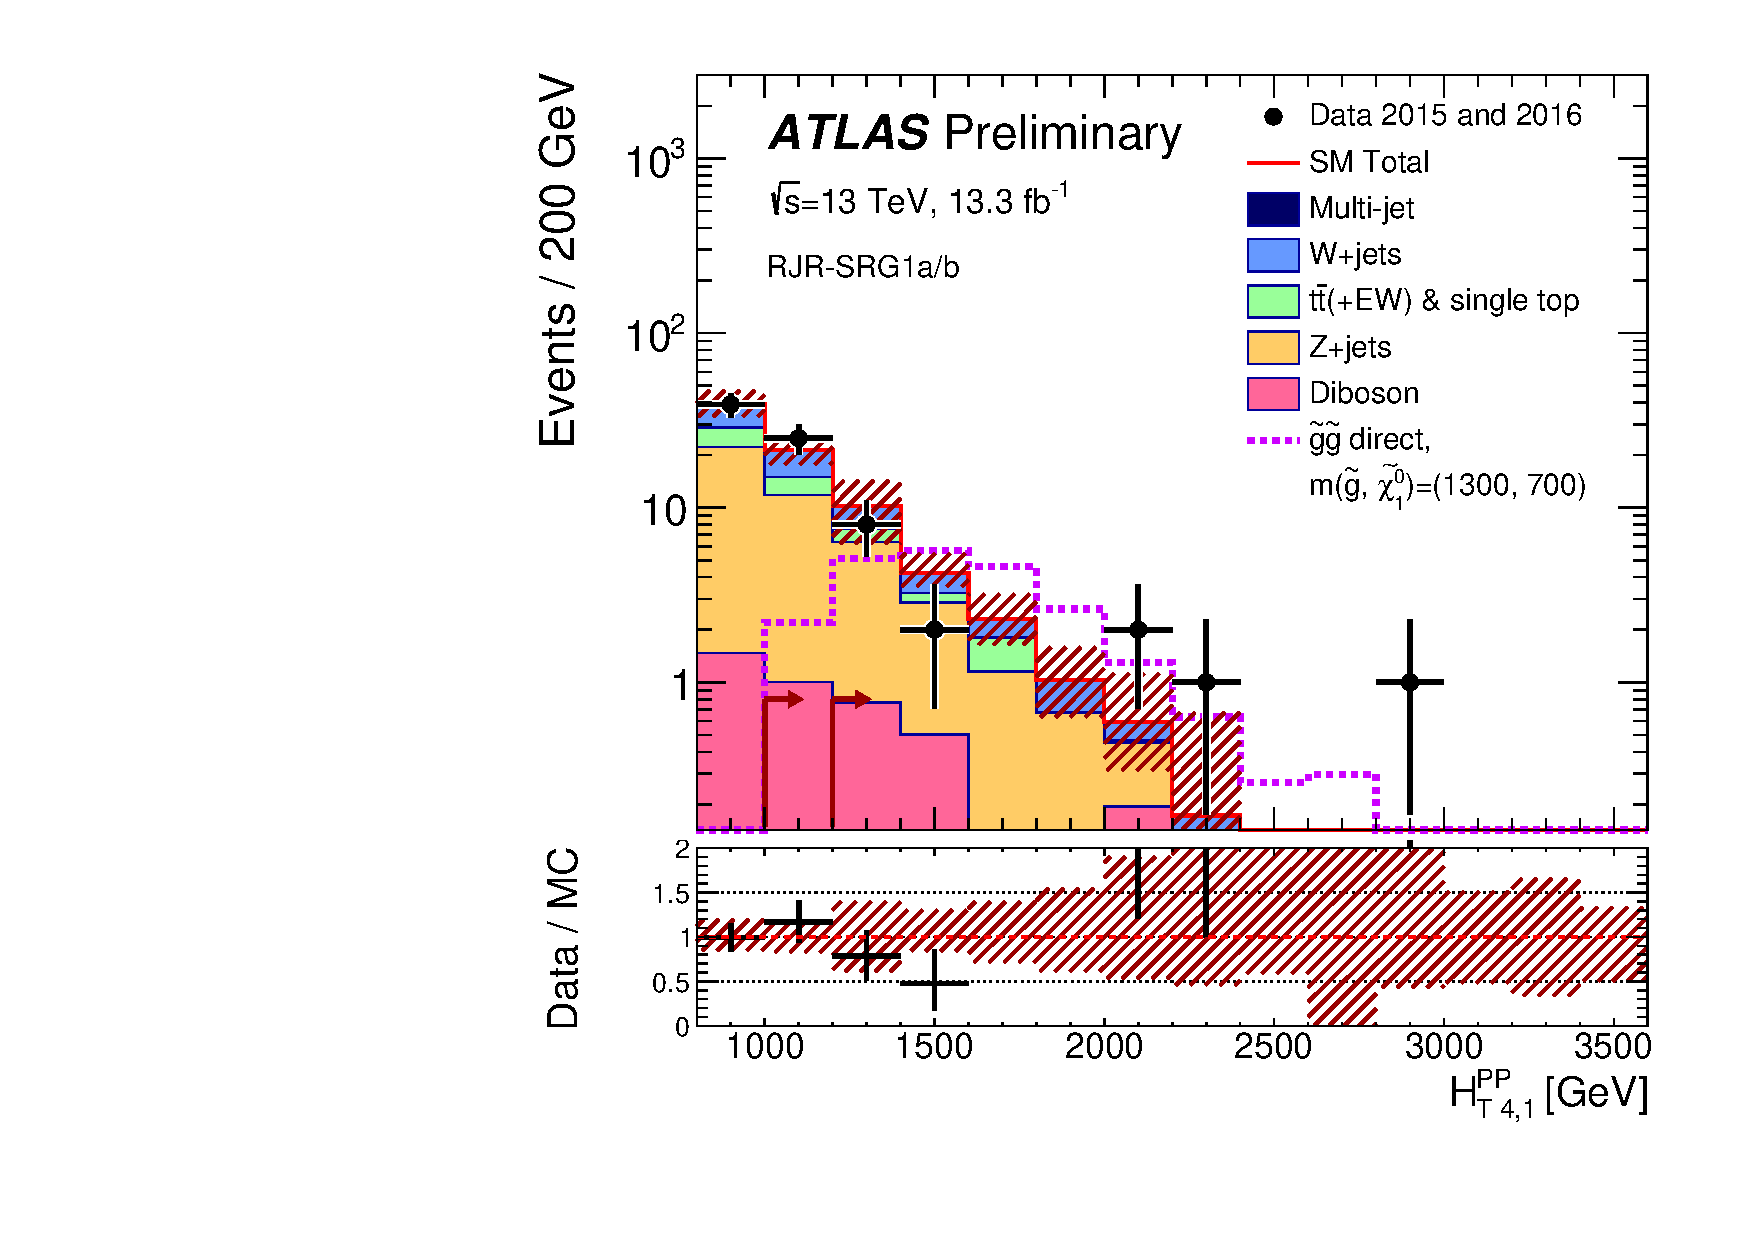
\includegraphics[width=0.45\textwidth]{ATLAS-CONF-2016-078_INT/N-1Plots/AtlasStyle/Preliminary/SR_SRJigsawSRG1a_LastCut_SR_minusone}
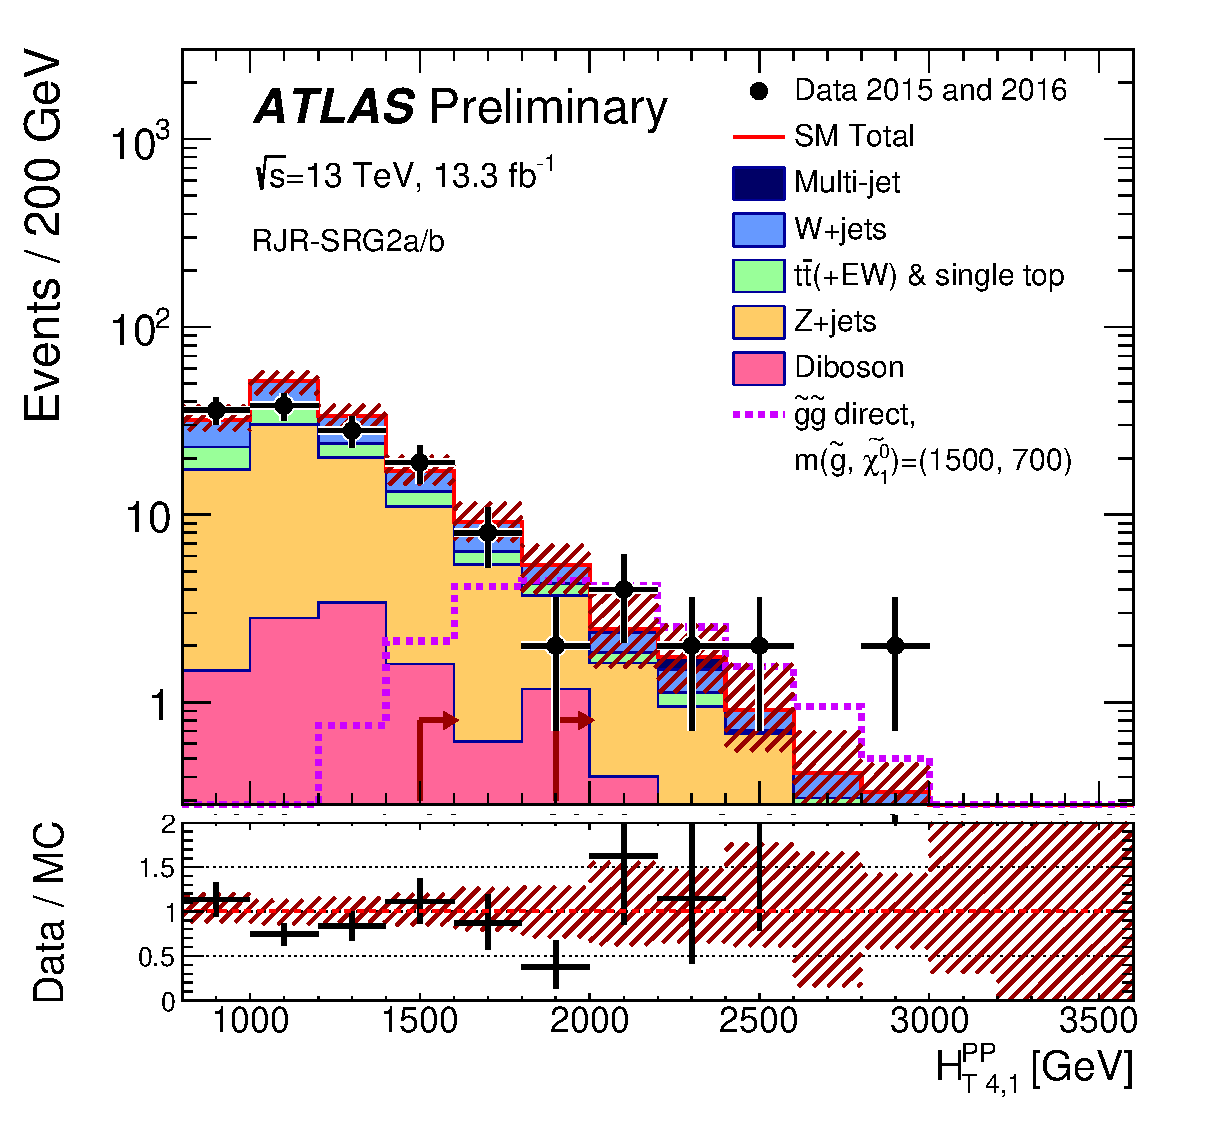
\includegraphics[width=0.45\textwidth]{ATLAS-CONF-2016-078_INT/N-1Plots/AtlasStyle/Preliminary/SR_SRJigsawSRG2a_LastCut_SR_minusone}
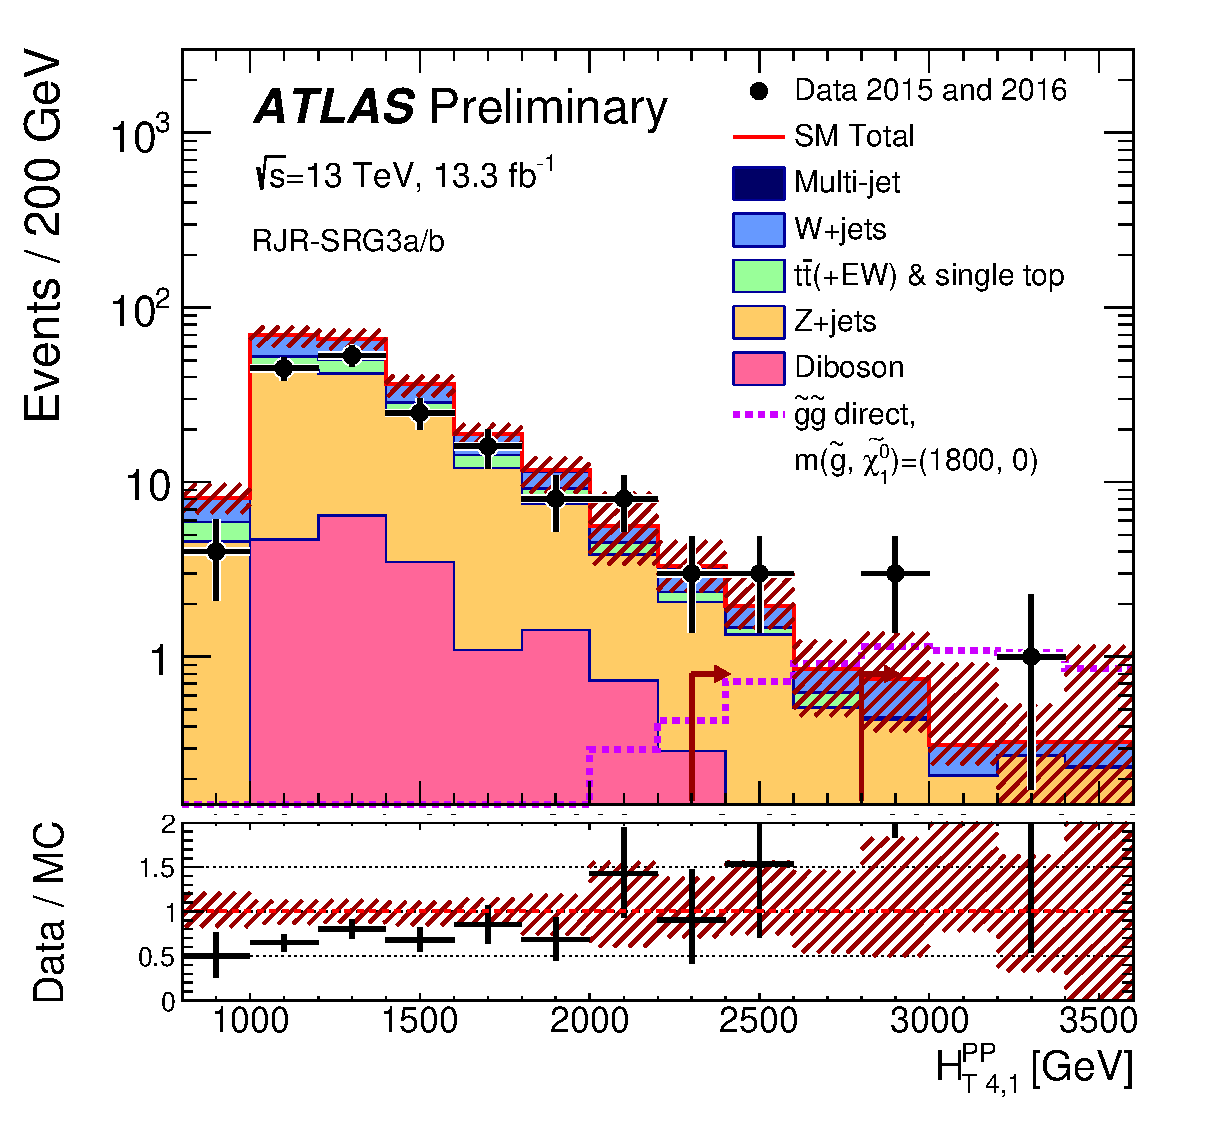
\includegraphics[width=0.45\textwidth]{ATLAS-CONF-2016-078_INT/N-1Plots/AtlasStyle/Preliminary/SR_SRJigsawSRG3a_LastCut_SR_minusone}
\end{center}
\caption{Scale variable distributions for the gluino signal regions.}
\label{fig:srg_scale}
\end{figure}

\begin{figure}[tbp]
\begin{center}
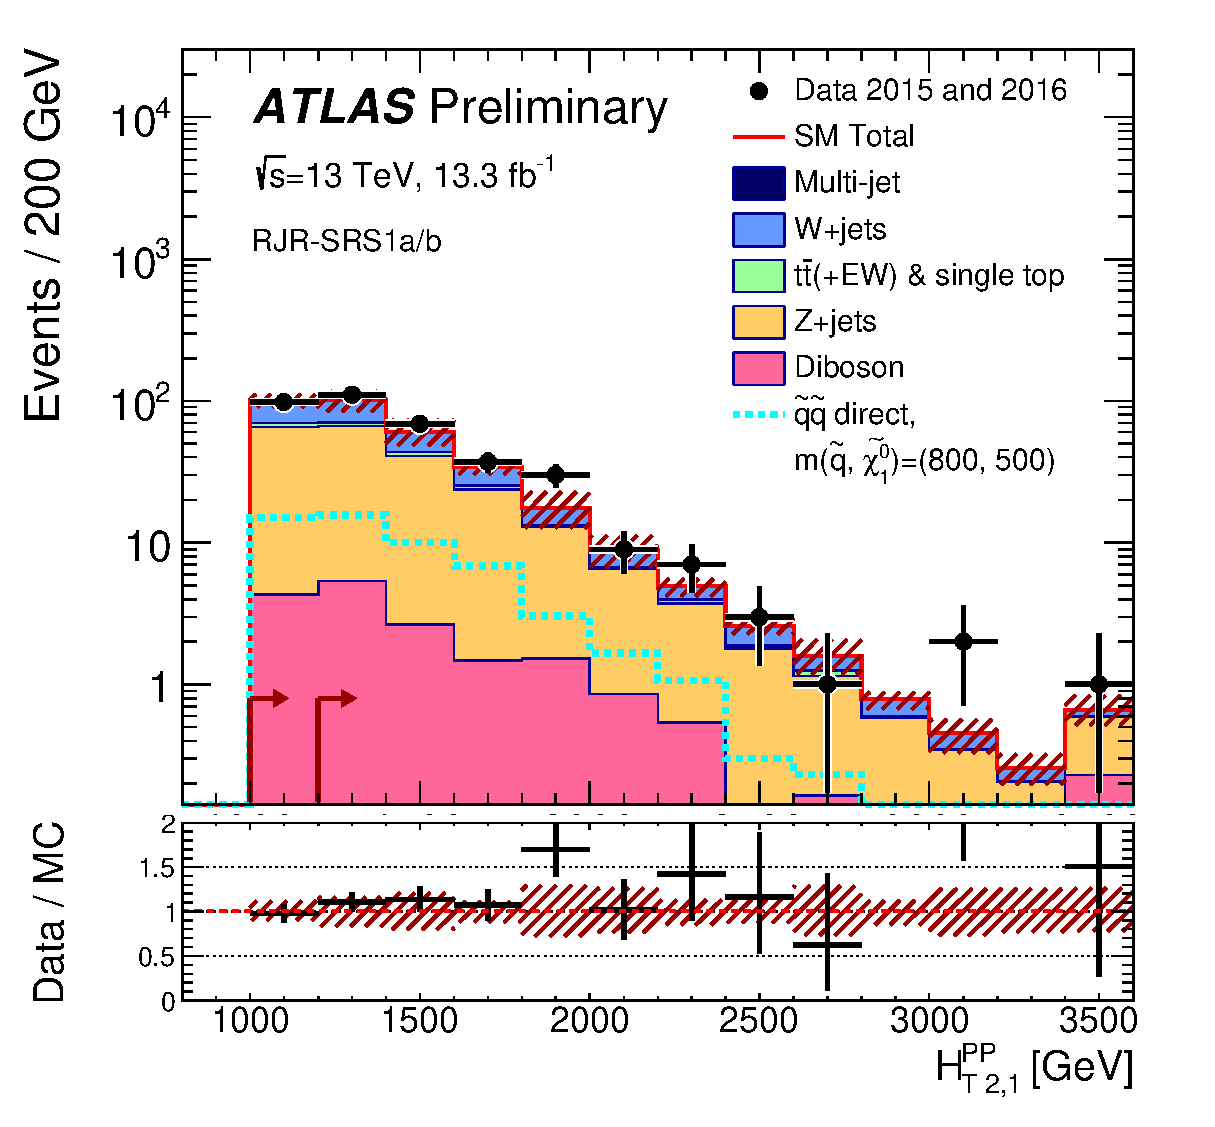
\includegraphics[width=0.45\textwidth]{ATLAS-CONF-2016-078_INT/N-1Plots/AtlasStyle/Preliminary/SR_SRJigsawSRS1a_LastCut_SR_minusone}
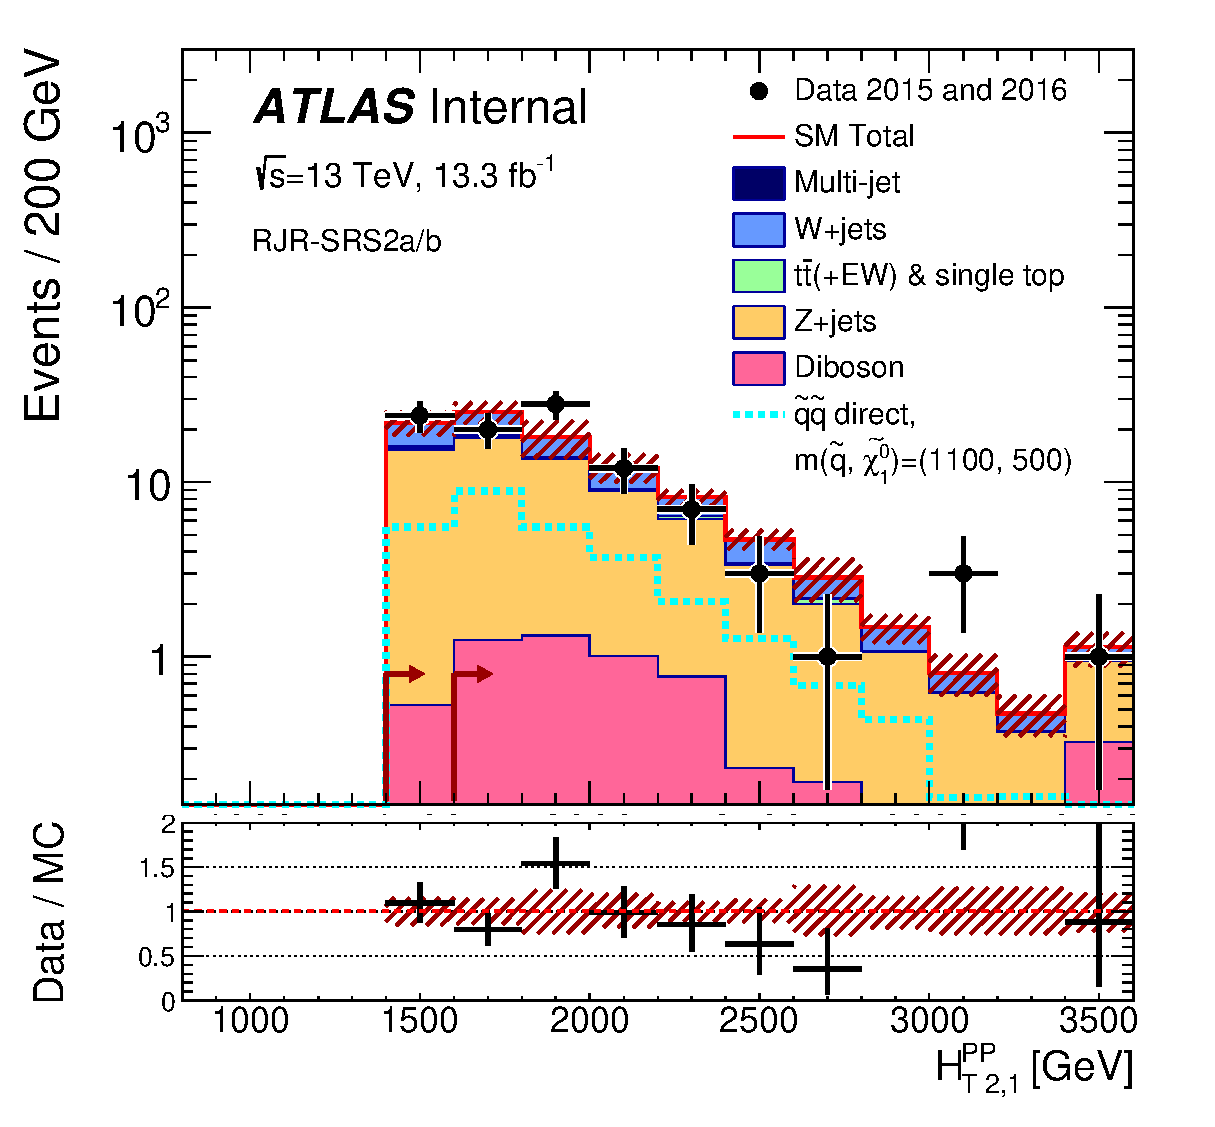
\includegraphics[width=0.45\textwidth]{ATLAS-CONF-2016-078_INT/N-1Plots/AtlasStyle/Preliminary/SR_SRJigsawSRS2a_LastCut_SR_minusone}
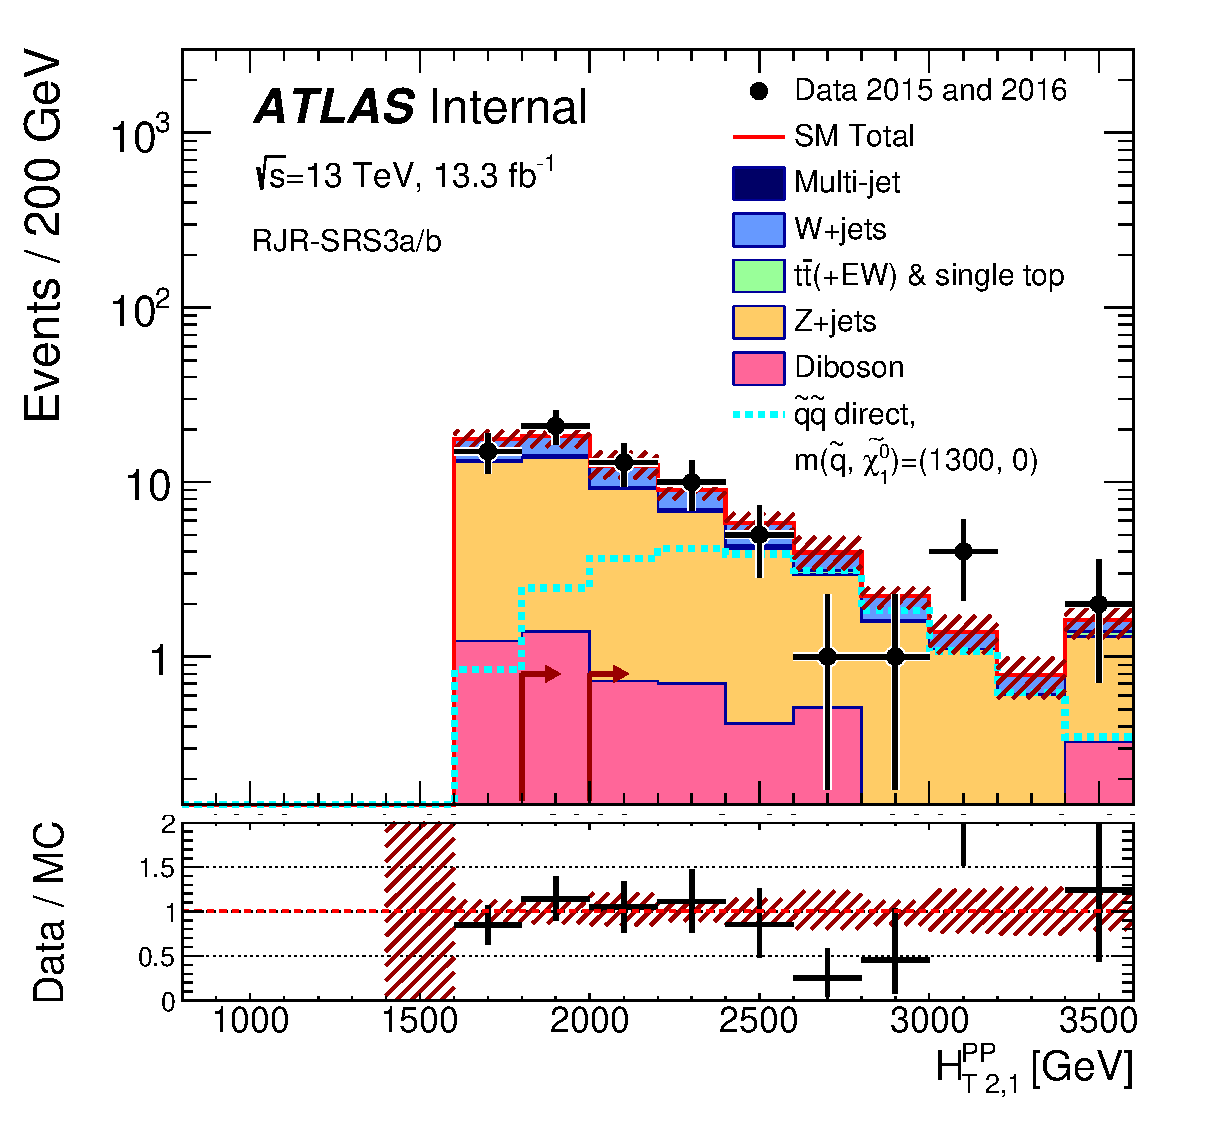
\includegraphics[width=0.45\textwidth]{ATLAS-CONF-2016-078_INT/N-1Plots/AtlasStyle/Preliminary/SR_SRJigsawSRS3a_LastCut_SR_minusone}
\end{center}
\caption{Scale variable distributions for the squark signal regions.}
\label{fig:srs_scale}
\end{figure}

\begin{figure}[tbp]
\begin{center}
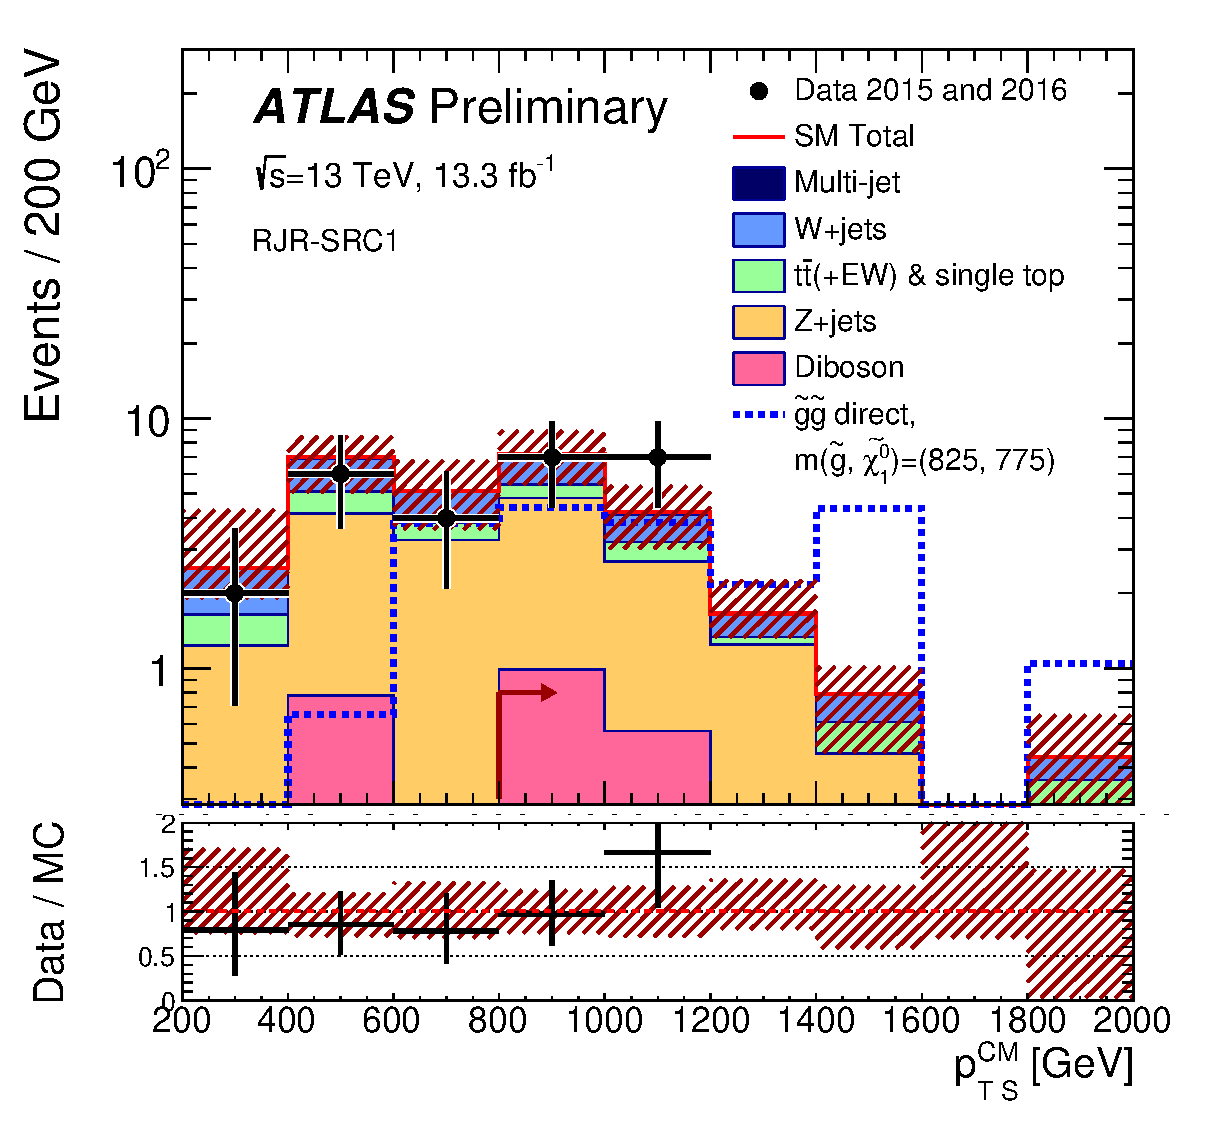
\includegraphics[width=0.45\textwidth]{ATLAS-CONF-2016-078_INT/N-1Plots/AtlasStyle/Preliminary/SR_SRJigsawSRC1_LastCut_SR_minusone}
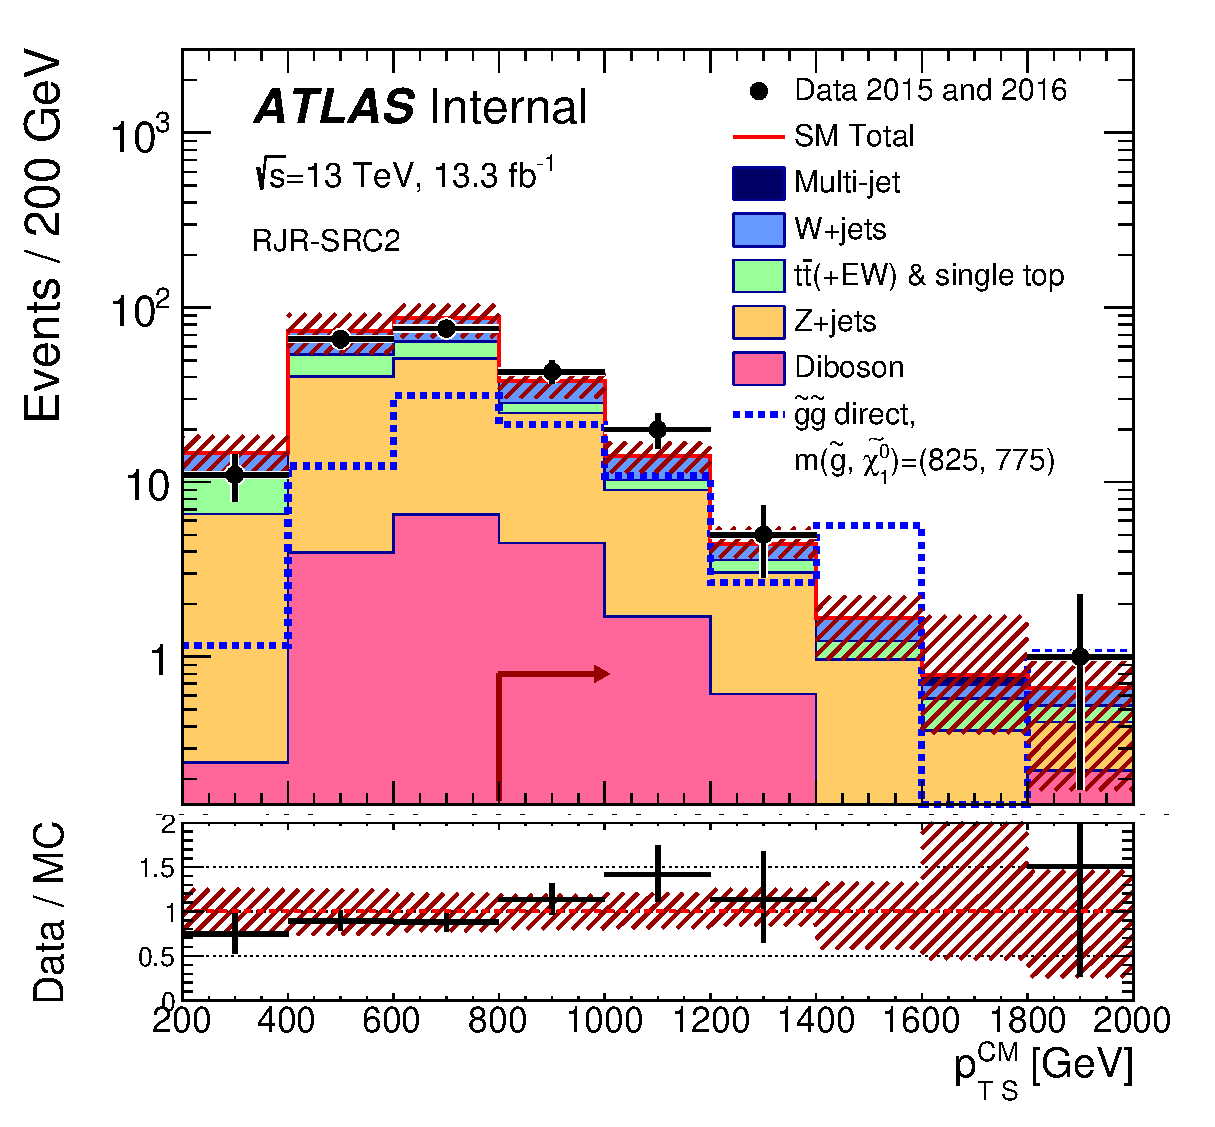
\includegraphics[width=0.45\textwidth]{ATLAS-CONF-2016-078_INT/N-1Plots/AtlasStyle/Preliminary/SR_SRJigsawSRC2_LastCut_SR_minusone}
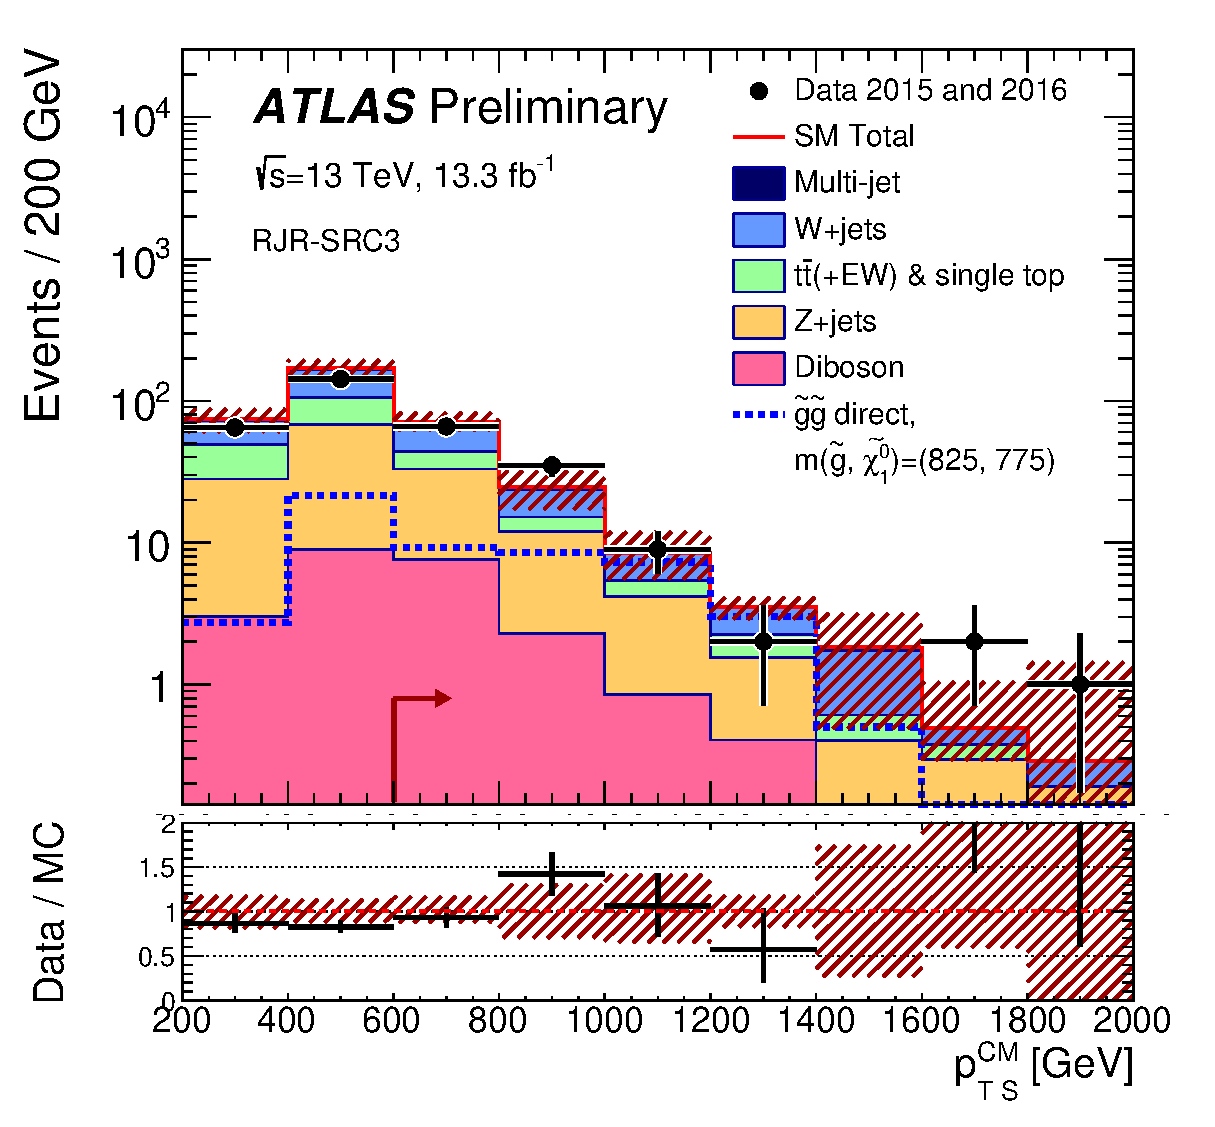
\includegraphics[width=0.45\textwidth]{ATLAS-CONF-2016-078_INT/N-1Plots/AtlasStyle/Preliminary/SR_SRJigsawSRC3_LastCut_SR_minusone}
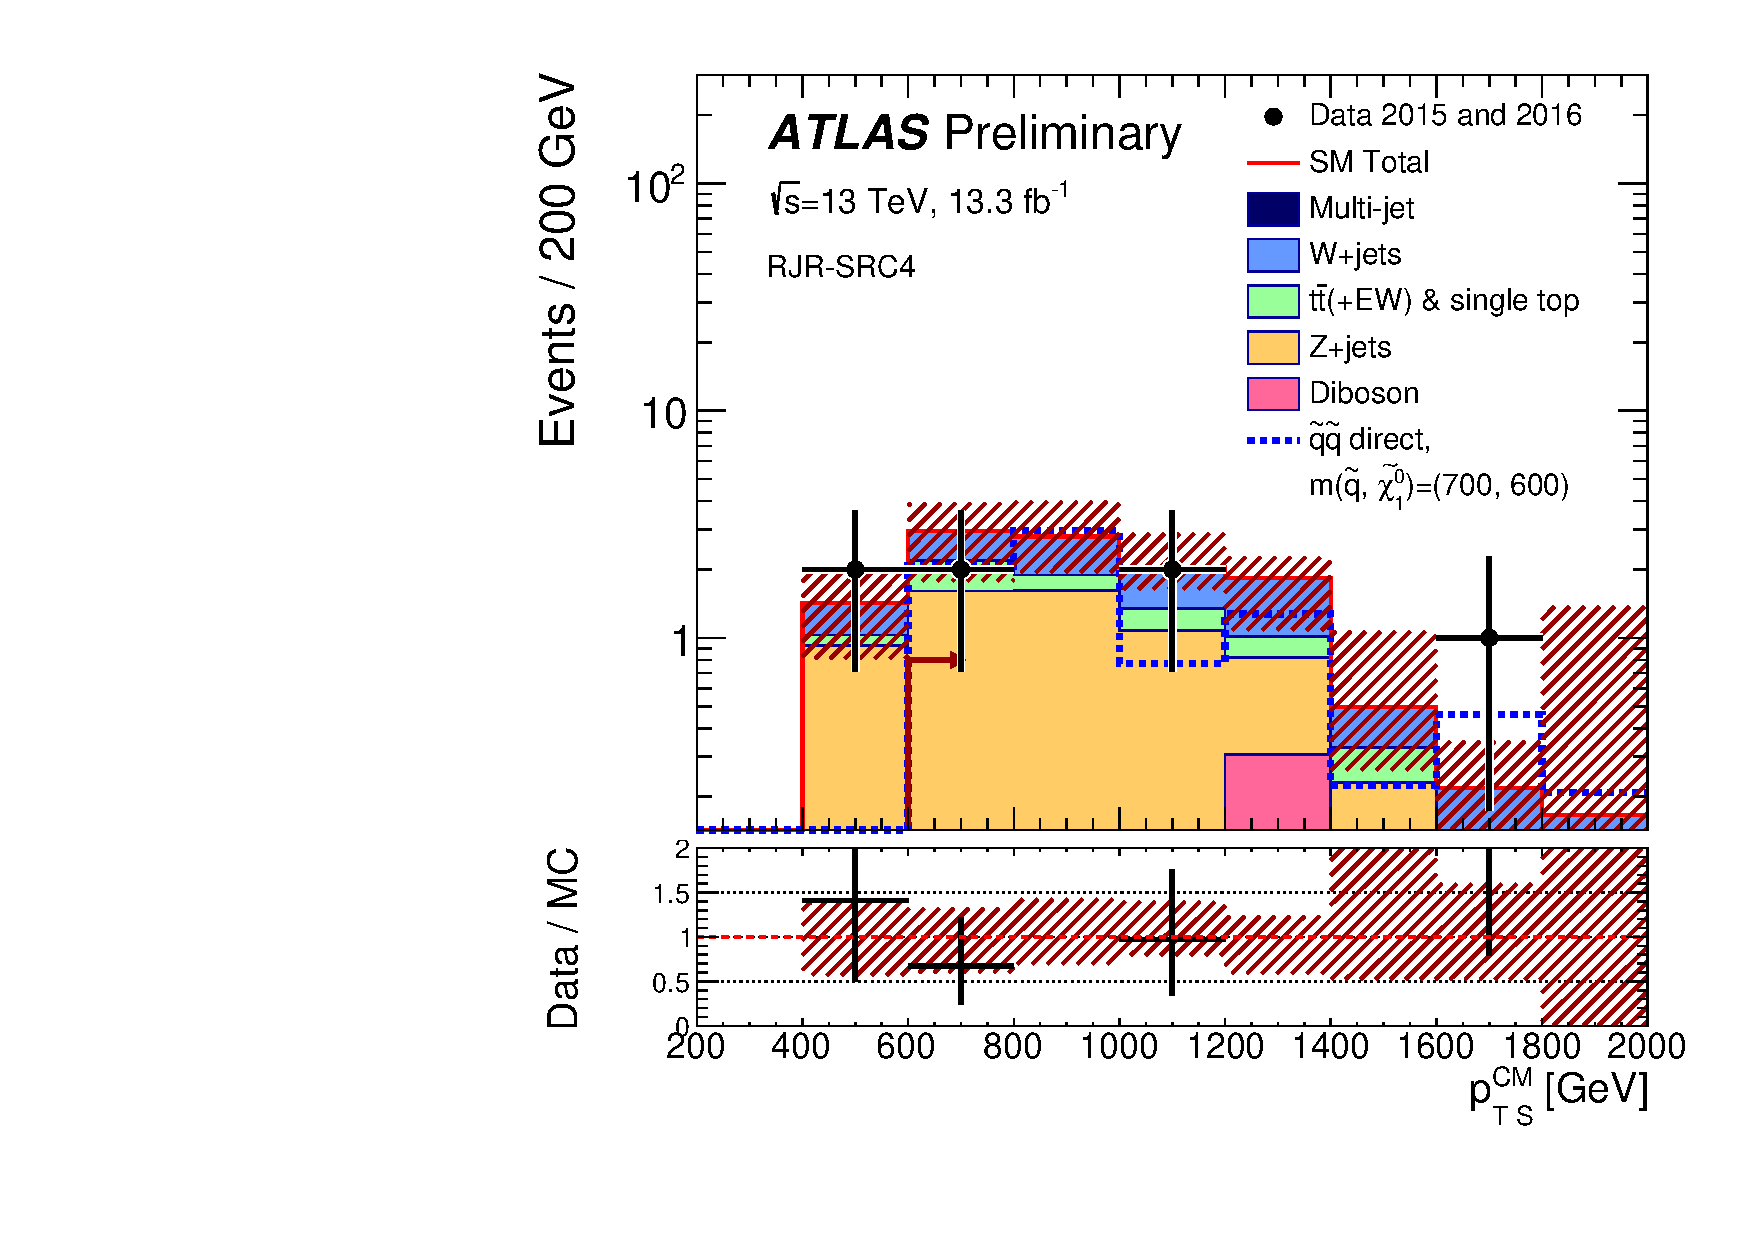
\includegraphics[width=0.45\textwidth]{ATLAS-CONF-2016-078_INT/N-1Plots/AtlasStyle/Preliminary/SR_SRJigsawSRC4_LastCut_SR_minusone}
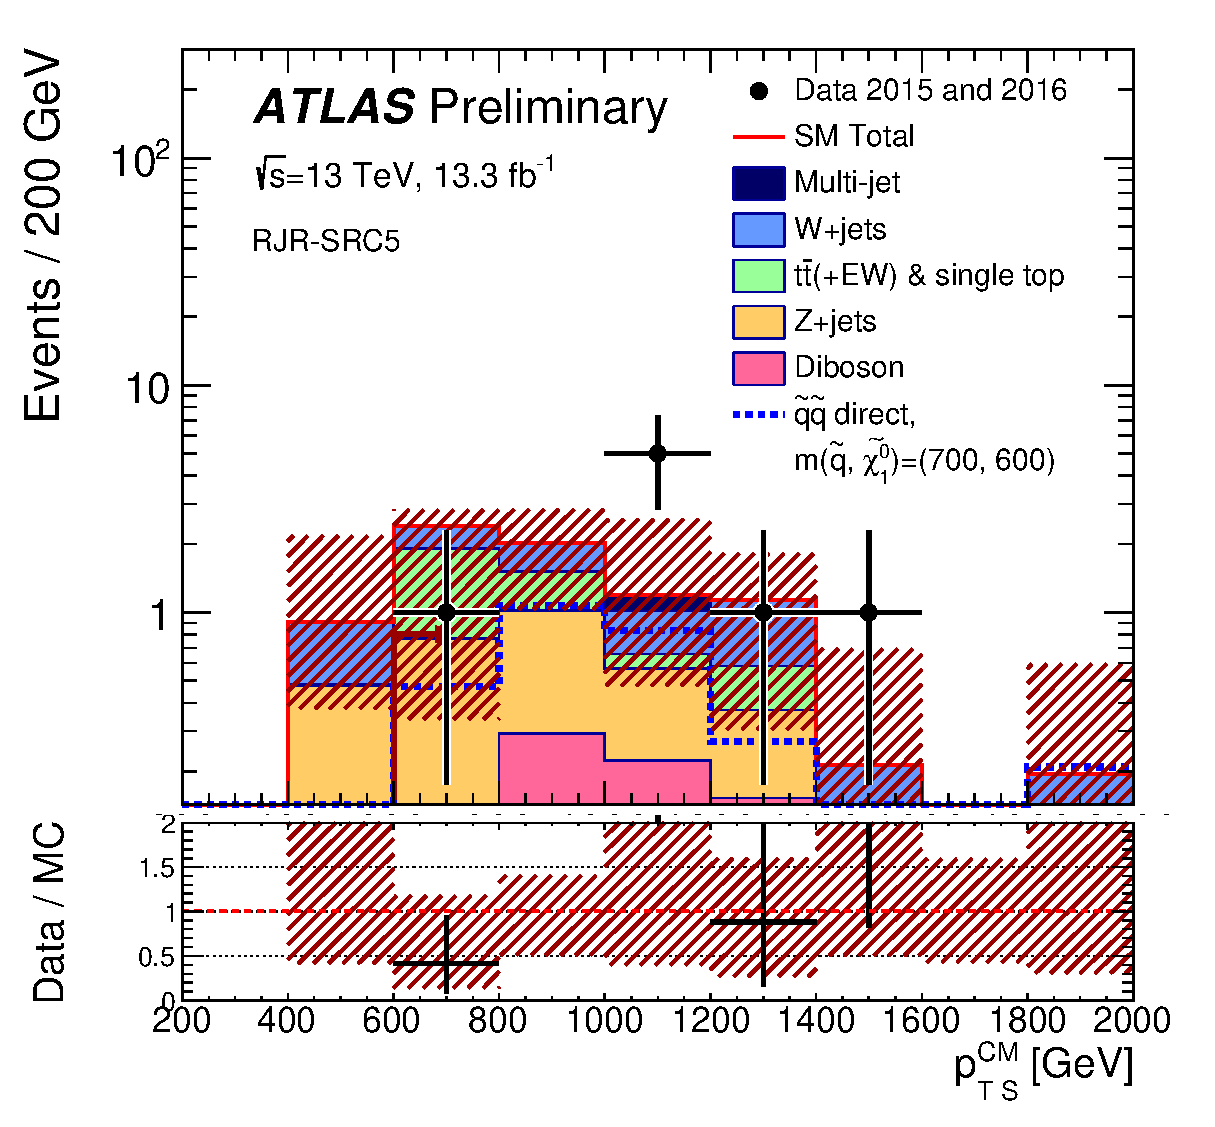
\includegraphics[width=0.45\textwidth]{ATLAS-CONF-2016-078_INT/N-1Plots/AtlasStyle/Preliminary/SR_SRJigsawSRC5_LastCut_SR_minusone}
\end{center}
\caption{Scale variable distributions for the compressed signal regions.}
\label{fig:src_scale}
\end{figure}


\Cref{fig:srs_scale,fig:srg_scale,fig:src_scale} show the unblinded distributions of the last scale cut  (\ptisr, \HTFnm{PP}{4}{1}, or \HTFnm{PP}{2}{1}) used for each signal region.
These distributions include the $\mu$ normalization scale factors for each SM background $\mu_B$ derived from the background-only fits.
The systematic uncertainties are also shown with a red dashed band.
In each plot, the distribution of one particular signal model is shown.
The signal model is targeted by the signal region shown in the plot, but each signal region targets a number of other signal models as well.
These distributions are shown after all signal region cuts are applied, except for the main scale variable shown on the horizontal axis.
We show the (a) and (b) version of a given noncompressed signal region on the same figure, as they differ only in the value of the main scale cut.
For example, SRS1a and SRS1b are both shown in the distribution of \HTFnm{PP}{2}{1} shown in the upper-left plot of \Cref{fig:srs_scale}.
The left (right) arrow shown is the location of the a (b) cut applied in the analysis.
We call these plot \textit{$N-1$} plots, where $N$ refers to the number of cuts applied in the analysis.

An expanded set of $N-1$ plots are available in \Cref{app:n-1_plots}.
Each variable which is used to discriminate signal from background has an associated $N-1$ plot.
These plots show the additional discrimination resulting from \textit{only} from the variable displayed on the horizontal axis.

\begin{figure}[tbp]
\centering
\caption{Summary of the signal regions} \label{fig:sr_summary}
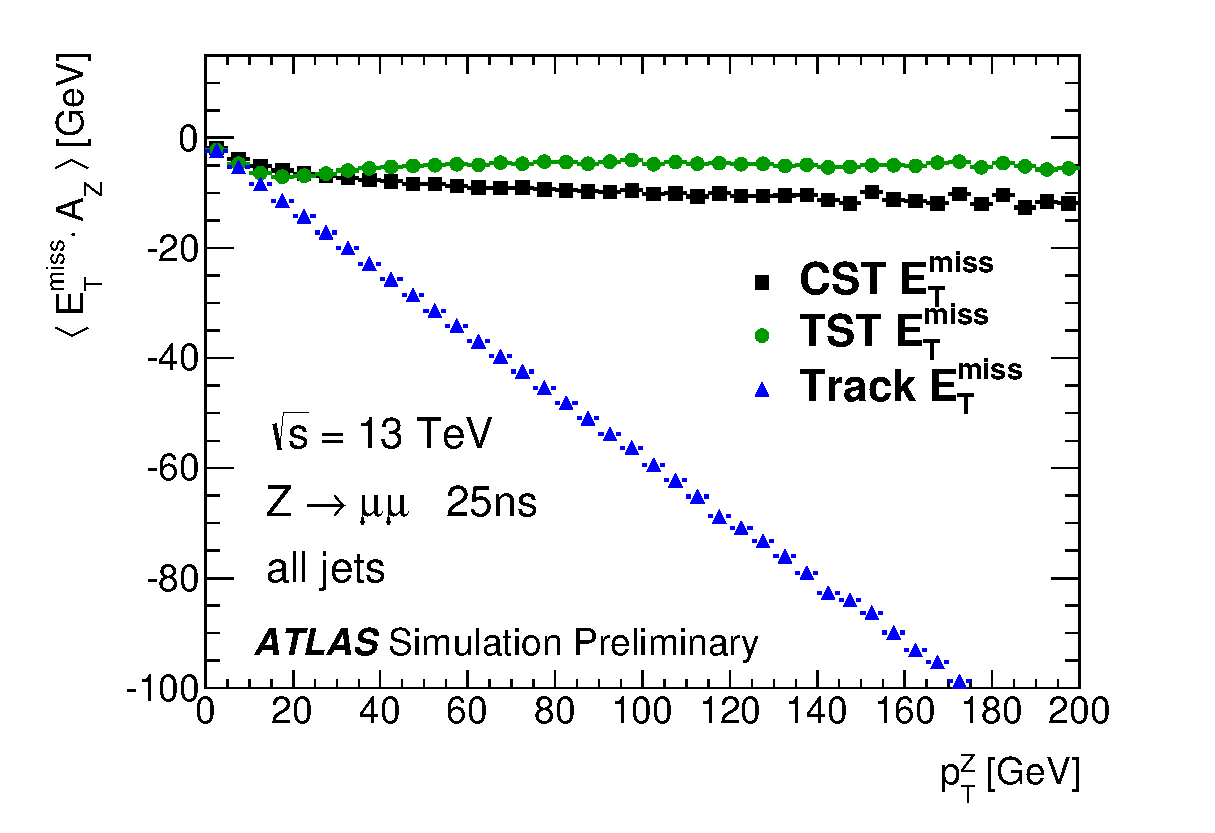
\includegraphics[width=.9\linewidth]{ATLAS-CONF-2016-078/fig_06b}
\end{figure}
A summary figure is shown in \Cref{fig:sr_summary}.
This figure shows the data and simulation event yields with the corresponding statistical and systematic uncertainties for all signal regions simultaneously.
%From this plot, we can see there is no significant excess of events over the Standard Model background.
This information is also presented in \Cref{tab:p0_UL_RJR}.
The table also includes the raw event yields from simulation before applying the $\mu$ normalization factor for comparison.
The model-independent limits are shown in this table.
\begin{table}[tbp]
\tiny
%\small
\begin{center}
\vspace*{-0.035\textwidth}
\begin{tabular}{|lrrrrrr|}
\hline
Signal Region & \textbf{ S1a } & \textbf{ S1b } & \textbf{ S2a } & \textbf{ S2b } & \textbf{ S3a } & \textbf{ S3b } \\
\hline
\multicolumn{7}{|c|}{MC expected events} \\ \hline
Diboson &  $17$               &  $13$               &  $5.6$               &  $5.1$               &  $4.2$               &  $2.8$               \\
$\mathrm{Z/\gamma^{*}}$+jets &  $231$               &  $163$               &  $63$               &  $48$               &  $36$               &  $24$               \\
W+jets &  $97$               &  $66$               &  $22$               &  $16$               &  $11$               &  $7.8$               \\
$\ttbar$(+EW) + single top &  $15$               &  $10$               &  $2.9$               &  $2.1$               &  $1.7$               &  $1.1$               \\
%%Multi-jet &  $0.93$               &  $0.53$               &  $0.13$               &  $0.00$               &  $0.00$               &  $0.00$               \\
\hline
\multicolumn{7}{|c|}{Fitted background events} \\ \hline
Diboson & $17 \pm 9$ & $13 \pm 7$ & $5.6 \pm 2.8$ & $5.1 \pm 2.6$ & $4.2 \pm 2.1$ & $2.8 \pm 1.4$ \\
$\mathrm{Z/\gamma^{*}}$+jets & $207 \pm 33$ & $146 \pm 23$ & $65 \pm 9$ & $50 \pm 7$ & $37 \pm 5$ & $25.0 \pm 3.5$ \\
W+jets & $95 \pm 9$ & $65 \pm 7$ & $24.1 \pm 2.9$ & $18.3 \pm 2.3$ & $12.8 \pm 2.8$ & $8.7 \pm 2.0$ \\
$\ttbar$(+EW) + single top & $14 \pm 7$ & $9 \pm 5$ & $2.1 \pm 1.7$ & $1.6 \pm 1.3$ & $1.3 \pm 1.0$ & $0.8 \pm 0.7$ \\
Multi-jet &  $0.71_{-0.71}^{+0.71}$               &  $0.41_{-0.41}^{+0.41}$               &  $0.08_{-0.08}^{+0.09}$               & -- & -- & -- \\
\hline
Total Expected MC &  $362$               &  $253$               &  $93$               &  $72$               &  $53$               &  $36$               \\
\hline
Total Fitted bkg & $334 \pm 35$ & $233 \pm 25$ & $96 \pm 10$ & $75 \pm 8$ & $56 \pm 6$ & $37 \pm 4$ \\
\hline
Observed &  $368$                     &  $270$                     &  $99$                     &  $75$                     &  $57$                     &  $36$                     \\
\hline


$\langle\epsilon\mathrm{ \sigma}\rangle_\mathrm{ obs}^{95}$ [fb]   &$7.6$  & $6.5$  & $2.2$  & $1.7$ & $1.6$ & $1.1$ \\
$S_\mathrm{ obs}^{95}$     & $101$ & $86$ & $29$ &  $23$ & $22$ & $15$ \\
$S_\mathrm{ exp}^{95}$     & $ { 78 }^{ +27 }_{ -21 }$ & $ { 61 }^{ +22 }_{ -16 }$ & $ { 28 }^{ +11 }_{ -8 }$ & $ { 23}^{ +9}_{ -7 }$ & $ { 20 }^{ +8 }_{ -6 }$ & $ { 16 }^{ +7 }_{ -5 }$  \\
$p_{0}$ ($\mathrm{Z}$)        & $ 0.20$~$(0.84)$ & $ 0.12$~$(1.17)$ & $ 0.44$~$(0.15)$& $ 0.50$~$(0.00)$ &  $ 0.44$~$(0.14)$ &  $ 0.50$~$(0.00)$ \\
\hline
\end{tabular}

% SRJigsawSRS1a    & $7.61$ &  $101.1$ & $ { 78.3 }^{ +27.0 }_{ -21.1 }$ & $0.00$ & $ 0.20$~$(0.84)$ \\%
% SRJigsawSRS1b    & $6.49$ &  $86.2$ & $ { 60.8 }^{ +22.2 }_{ -16.4 }$ & $0.87$ & $ 0.12$~$(1.17)$ \\%
% SRJigsawSRS2a    & $2.20$ &  $29.3$ & $ { 27.8 }^{ +10.9 }_{ -7.8 }$ & $0.56$ & $ 0.44$~$(0.15)$ \\%
% SRJigsawSRS2b    & $1.72$ &  $22.9$ & $ { 23.4 }^{ +9.4 }_{ -6.5 }$ & $0.47$ & $ 0.50$~$(0.00)$ \\% %% NOTE: capped p-value was nan, wrote 0.5 since nObs < nExp
% SRJigsawSRS3a    & $1.62$ &  $21.5$ & $ { 20.4 }^{ +8.4 }_{ -5.8 }$ & $0.56$ & $ 0.44$~$(0.14)$ \\%
% SRJigsawSRS3b    & $1.14$ &  $15.1$ & $ { 16.0 }^{ +6.7 }_{ -4.5 }$ & $0.44$ & $ 0.49$~$(0.03)$ \\%


%\vspace{0.5cm}
%\end{center}
%\end{table}
\begin{tabular}{|lrrrrrr|}
\hline
Signal Region & \textbf{ G1a } & \textbf{ G1b } & \textbf{ G2a } & \textbf{ G2b } & \textbf{ G3a } & \textbf{ G3b } \\
\hline
\multicolumn{7}{|c|}{MC expected events} \\ \hline
Diboson &  $2.6$               &  $1.6$               &  $2.9$               &  $1.1$               &  $0.62$               &  $0.26$               \\
$\mathrm{Z/\gamma^{*}}$+jets &  $18$               &  $8.8$               &  $13$               &  $4.2$               &  $3.1$               &  $0.83$               \\
W+jets &  $11$               &  $4.7$               &  $7.7$               &  $2.0$               &  $1.9$               &  $0.63$               \\
$\ttbar$(+EW) + single top &  $7.4$               &  $3.1$               &  $4.4$               &  $1.1$               &  $0.34$               &  $0.03$               \\
%%Multi-jet &  $0.27$               &  $0.13$               &  $0.53$               &  $0.40$               &  $0.00$               &  $0.00$               \\
\hline
\multicolumn{7}{|c|}{Fitted background events} \\ \hline
Diboson & $2.6 \pm 1.3$ & $1.6 \pm 0.8$ & $2.9 \pm 1.5$ & $1.1 \pm 0.6$ & $0.6 \pm 0.4$ & $0.26 \pm 0.14$ \\
$\mathrm{Z/\gamma^{*}}$+jets & $21.1 \pm 3.1$ & $10.2 \pm 1.6$ & $14.3 \pm 2.5$ & $4.5 \pm 0.8$ & $3.3 \pm 0.6$ & $0.88 \pm 0.19$ \\
W+jets & $10.8 \pm 1.7$ & $4.6 \pm 1.4$ & $6.7 \pm 1.3$ & $1.7 \pm 0.7$ & $1.6 \pm 0.7$ & $0.55 \pm 0.2$ \\
$\ttbar$(+EW) + single top & $5.4 \pm 1.6$ & $2.3 \pm 0.9$ & $3.4 \pm 1.4$ & $0.8 \pm 0.5$ &  $0.26_{-0.26}^{+0.45}$               &  $0.02_{-0.02}^{+0.26}$               \\
Multi-jet & $0.24 \pm 0.24$ & $0.12 \pm 0.12$ & $0.5 \pm 0.5$ & $0.4 \pm 0.4$ & -- & -- \\
\hline
Total Expected MC &  $39$               &  $18$               &  $29$               &  $8.7$               &  $5.9$               &  $1.7$               \\
\hline
Total Fitted bkg & $40 \pm 4$ & $18.8 \pm 2.5$ & $27.8 \pm 3.4$ & $8.5 \pm 1.4$ & $5.8 \pm 1.1$ & $1.7 \pm 0.4$ \\
\hline
Observed &  $39$                     &  $14$                     &  $30$                     &  $10$                     &  $8$                     &  $4$                     \\
\hline


$\langle\epsilon\mathrm{ \sigma}\rangle_\mathrm{ obs}^{95}$ [fb]   & $1.1$   &  $0.56$  &  $1.1$ & $0.71$ & $0.64$ &  $0.55$ \\
$S_\mathrm{ obs}^{95}$     & $15$ & $7.5$ &$15$ & $9.4$ & $8.5$  &  $7.3$ \\
$S_\mathrm{ exp}^{95}$     & $ { 16 }^{ +7 }_{ -4 }$  & $ { 10 }^{ +5 }_{ -3 }$ & $ { 14 }^{ +6 }_{ -4 }$ & $ { 7.6 }^{ +3.5}_{ -2.0 }$ & $ { 7.0 }^{ +2.5}_{ -2.1 }$  & $ { 4.2 }^{ +1.9 }_{ -0.5 }$\\
$p_{0}$ ($\mathrm{Z}$)        & $ 0.50$~$(0.00)$  & $ 0.50$~$(0.00)$ & $ 0.36$~$(0.35)$ & $ 0.31$~$(0.50)$ & $ 0.21$~$(0.81)$ & $ 0.06$~$(1.55)$ \\
\hline
\end{tabular}


% SRJigsawSRG1a    & $1.13$ &  $15.0$ & $ { 15.7 }^{ +6.7 }_{ -4.4 }$ & $0.45$ & $ 0.50$~$(0.00)$ \\% %% NOTE: capped p-value was nan, wrote 0.5 since nObs < nExp
% SRJigsawSRG1b    & $0.56$ &  $7.5$ & $ { 10.3 }^{ +4.8 }_{ -2.9 }$ & $0.18$ & $ 0.50$~$(0.00)$ \\%
% SRJigsawSRG2a    & $1.14$ &  $15.2$ & $ { 13.6 }^{ +5.8 }_{ -3.9 }$ & $0.63$ & $ 0.36$~$(0.35)$ \\%
% SRJigsawSRG2b    & $0.70$ &  $9.3$ & $ { 7.7 }^{ +4.0 }_{ -2.3 }$ & $0.65$ & $ 0.33$~$(0.44)$ \\%
% SRJigsawSRG3a    & $0.67$ &  $8.9$ & $ { 7.1 }^{ +3.0 }_{ -2.2 }$ & $0.73$ & $ 0.23$~$(0.74)$ \\%
% SRJigsawSRG3b    & $0.56$ &  $7.5$ & $ { 7.0 }^{ +2.7 }_{ -2.0 }$ & $0.62$ & $ 0.18$~$(0.93)$ \\%


%\end{center}
%\end{table}
\begin{tabular}{|lrrrrr|}
\hline
Signal Region & \textbf{ C1 } & \textbf{ C2 } & \textbf{ C3 } & \textbf{ C4 } & \textbf{ C5 } \\
\hline
\multicolumn{6}{|c|}{MC expected events} \\ \hline
Diboson &  $1.9$               &  $7.1$               &  $11$               &  $0.54$               &  $0.75$               \\
$\mathrm{Z/\gamma^{*}}$+jets &  $8.8$               &  $36$               &  $46$               &  $5.8$               &  $2.5$               \\
W+jets &  $3.5$               &  $16$               &  $43$               &  $3.8$               &  $2.3$               \\
$\ttbar$(+EW) + single top &  $1.9$               &  $7.2$               &  $20$               &  $1.7$               &  $2.5$               \\
%%Multi-jet &  $0.13$               &  $0.53$               &  $3.05$               &  $0.00$               &  $0.27$               \\
\hline
\multicolumn{6}{|c|}{Fitted background events} \\ \hline
Diboson & $1.9 \pm 1.0$ & $7 \pm 4$ & $11 \pm 6$ & $0.54 \pm 0.29$ & $0.8 \pm 0.5$ \\
$\mathrm{Z/\gamma^{*}}$+jets & $7.7 \pm 1.1$ & $32 \pm 5$ & $40 \pm 6$ & $5.0 \pm 0.8$ & $2.2 \pm 0.4$ \\
W+jets & $3.3 \pm 1.4$ & $14.5 \pm 1.7$ & $40 \pm 5$ & $3.56 \pm 1.0$ & $2.14 \pm 0.35$ \\
$\ttbar$(+EW) + single top & $1.5 \pm 0.6$ & $5.8 \pm 1.8$ & $16 \pm 5$ & $1.4 \pm 0.7$ & $2.0 \pm 1.1$ \\
Multi-jet & $0.09 \pm 0.09$ & $0.4 \pm 0.4$ & $2.1 \pm 2.1$ & -- & $0.18 \pm 0.18$ \\
\hline
Total Expected MC &  $16$               &  $67$               &  $124$               &  $12$               &  $8.3$               \\
\hline
Total Fitted bkg & $14.5 \pm 2.2$ & $59 \pm 6$ & $110 \pm 11$ & $10.5 \pm 1.5$ & $7.3 \pm 1.4$ \\
\hline
Observed &  $14$                     &  $69$                     &  $115$                     &  $5$                     &  $8$                     \\
\hline


$\langle\epsilon\mathrm{ \sigma}\rangle_\mathrm{ obs}^{95}$ [fb]   &$0.76$   & $2.2$ & $2.5$  & $0.35$ & $0.61$  \\
$S_\mathrm{ obs}^{95}$     & $10$ & $29$ &  $34$  & $4.7$ & $8.1$ \\
$S_\mathrm{ exp}^{95}$     & $ { 11 }^{ +5 }_{ -3 }$ &  $ { 21 }^{ +9 }_{ -6 }$ & $ { 30 }^{ +12 }_{ -8 }$ & $ { 8.1 }^{ +3.0 }_{ -2.3 }$ & $ { 7.4 }^{ +2.9 }_{ -1.8 }$ \\
$p_{0}$ ($\mathrm{Z}$)        & $ 0.50$~$(0.00)$  & $ 0.18$~$(0.92)$ & $ 0.37$~$(0.32)$ & $ 0.50$~$(0.00)$  & $ 0.39$~$(0.30)$ \\
\hline
\end{tabular}

% SRJigsawSRC1    & $0.76$ &  $10.1$ & $ { 10.6 }^{ +4.6 }_{ -3.1 }$ & $0.46$ & $ 0.50$~$(0.00)$ \\% %% NOTE: capped p-value was nan, wrote 0.5 since nObs < nExp
% SRJigsawSRC2    & $2.15$ &  $28.6$ & $ { 21.1 }^{ +8.7 }_{ -6.0 }$ & $0.81$ & $ 0.18$~$(0.92)$ \\%
% SRJigsawSRC3    & $2.52$ &  $33.5$ & $ { 30.2 }^{ +11.7 }_{ -8.4 }$ & $0.62$ & $ 0.37$~$(0.32)$ \\%
% SRJigsawSRC4    & $0.36$ &  $4.8$ & $ { 7.7 }^{ +4.0 }_{ -2.3 }$ & $0.06$ & $ 0.48$~$(0.06)$ \\%
% SRJigsawSRC5    & $0.61$ &  $8.1$ & $ { 7.5 }^{ +3.6 }_{ -2.4 }$ & $0.59$ & $ 0.41$~$(0.23)$ \\%

\vspace*{-0.01\textheight}\caption{Numbers of events observed in the signal regions compared with background expectations.
Empty cells (indicated by a `-') correspond to estimates lower than $0.01$.
% The p-values ($p_{0}$) give the probabilities of the observations being consistent with the estimated backgrounds.
% For an observed number of events lower than expected, the p-value is truncated at 0.5.
% Between parentheses, $p$-values are also given as the number of equivalent Gaussian standard deviations (Z).
Also shown are 95\% CL upper limits on the visible cross-section ($\langle\epsilon\sigma\rangle_\mathrm{ obs}^{95}$),
the visible number of signal events ($S_\mathrm{ obs}^{95}$ ) and the number of signal events ($S_\mathrm{ exp}^{95}$)
given the expected number of background events (and $\pm 1\sigma$ excursions of the expectation).
\label{tab:p0_UL_RJR}}
\end{center}
\end{table}


\section{Systematic Uncertainties}

This section considers the results of \Cref{tab:BreakdownSysSRCompressed_RJR}.
This table is a summary of the systematic uncertainties on the SM background event yields in each signal region.
These uncertainties are expressed both as relative and absolute uncertainties.
The absolute uncertainties do not add in quadrature as the uncertainties can be correlated.
%Example correlation matrices are shown for SRC1, SRG1a, and SRS1a in \Cref{}
%These show the pairwise correlation factors between each systematic uncertainty included in the fitting procedure \todo{remove ones that aren't actually in the tables}
We discuss the general trends in the systematic uncertainties for each type of signal region.

In the squark regions, the total uncertainties including statistical and systematic uncertainties range are approximately 10\% of the total event yield.
The uncertainties on the $Z$ event yields, both theoretical and $\Delta_{\mu,\mathrm{Z+jets}}$ are the largest uncertainties for each signal region.
The $\kappa$ factor uncertainty, which is also an uncertainty on the $Z$ event yield, is also significant at 4\% in each region.
The \Zvv contribution to the squark regions is the primary irreducible background, so even when relatively well-measured, the $Z$ event yield uncertainties dominate the overall background uncertainty.
There are also significant uncertainties from the $W$, top, and flat diboson uncertainties.
The uncertainty due to statistics of the MC simulation samples are small for the squark case; this is a reflection of the ``looseness'' of these regions.

The gluino regions have overall larger total uncertainties on the background event yields than the squark regions, from 10\% and 25\%.
The $Z$ uncertainties all contribute significantly, yet they are similar to the squark $Z$ event yield uncertainties.
The $W$, top, and diboson uncertainties are all significantly larger than in the squark case.
In the gluino case, we also see that the limited simulation statistics begin to significantly affect the estimation of the Standard Model background event yield.
These are all reflections of the overall ``tighter'' quality of the gluino regions.
%The $\Delta_{\mu}$ uncertainties are affected by the tightness of the regions due to the need to use overall looser control regions, which are
%The theory uncertainties are more affected by small statistical fluctuations between different generators when
In SRG3b, the low simulation statistics account for a large 14\% statistical uncertainty on the SR event yields.\todo{actually check this stuff and maybe reinclude stuff}

The compressed regions have systematic uncertainties ranging from 10\% to 19\%.\todo{look back at Emlyn's notes}
For the tighter regions, SRC1, SRC4, and SRC5, there is a large contribution owing to a lack of MC statistics.
SRC1 and SRC4 should a large value for the $W$ theory uncertainty, while all compressed regions show a large uncertainty on the $Z$ estimate.
These large uncertainties result from the fact that we are probing extreme phase space in boson \pt with the compressed regions.
SRC5 shows large top and jet/\met uncertainties; these uncertainties are more pronounced in this region than the other compressed region due to the $\NVjet > 3$ cut, and thus the uncertainty in this region is quite affected by fluctuations in the top, jet, or \met uncertainties.

% \begin{figure}[tbph]
% \centering
% \caption{Correlation factors between systematic uncertainties in SRC1, SRG1a, and SRS1a.} \label{fig:systematic_correlations}
% 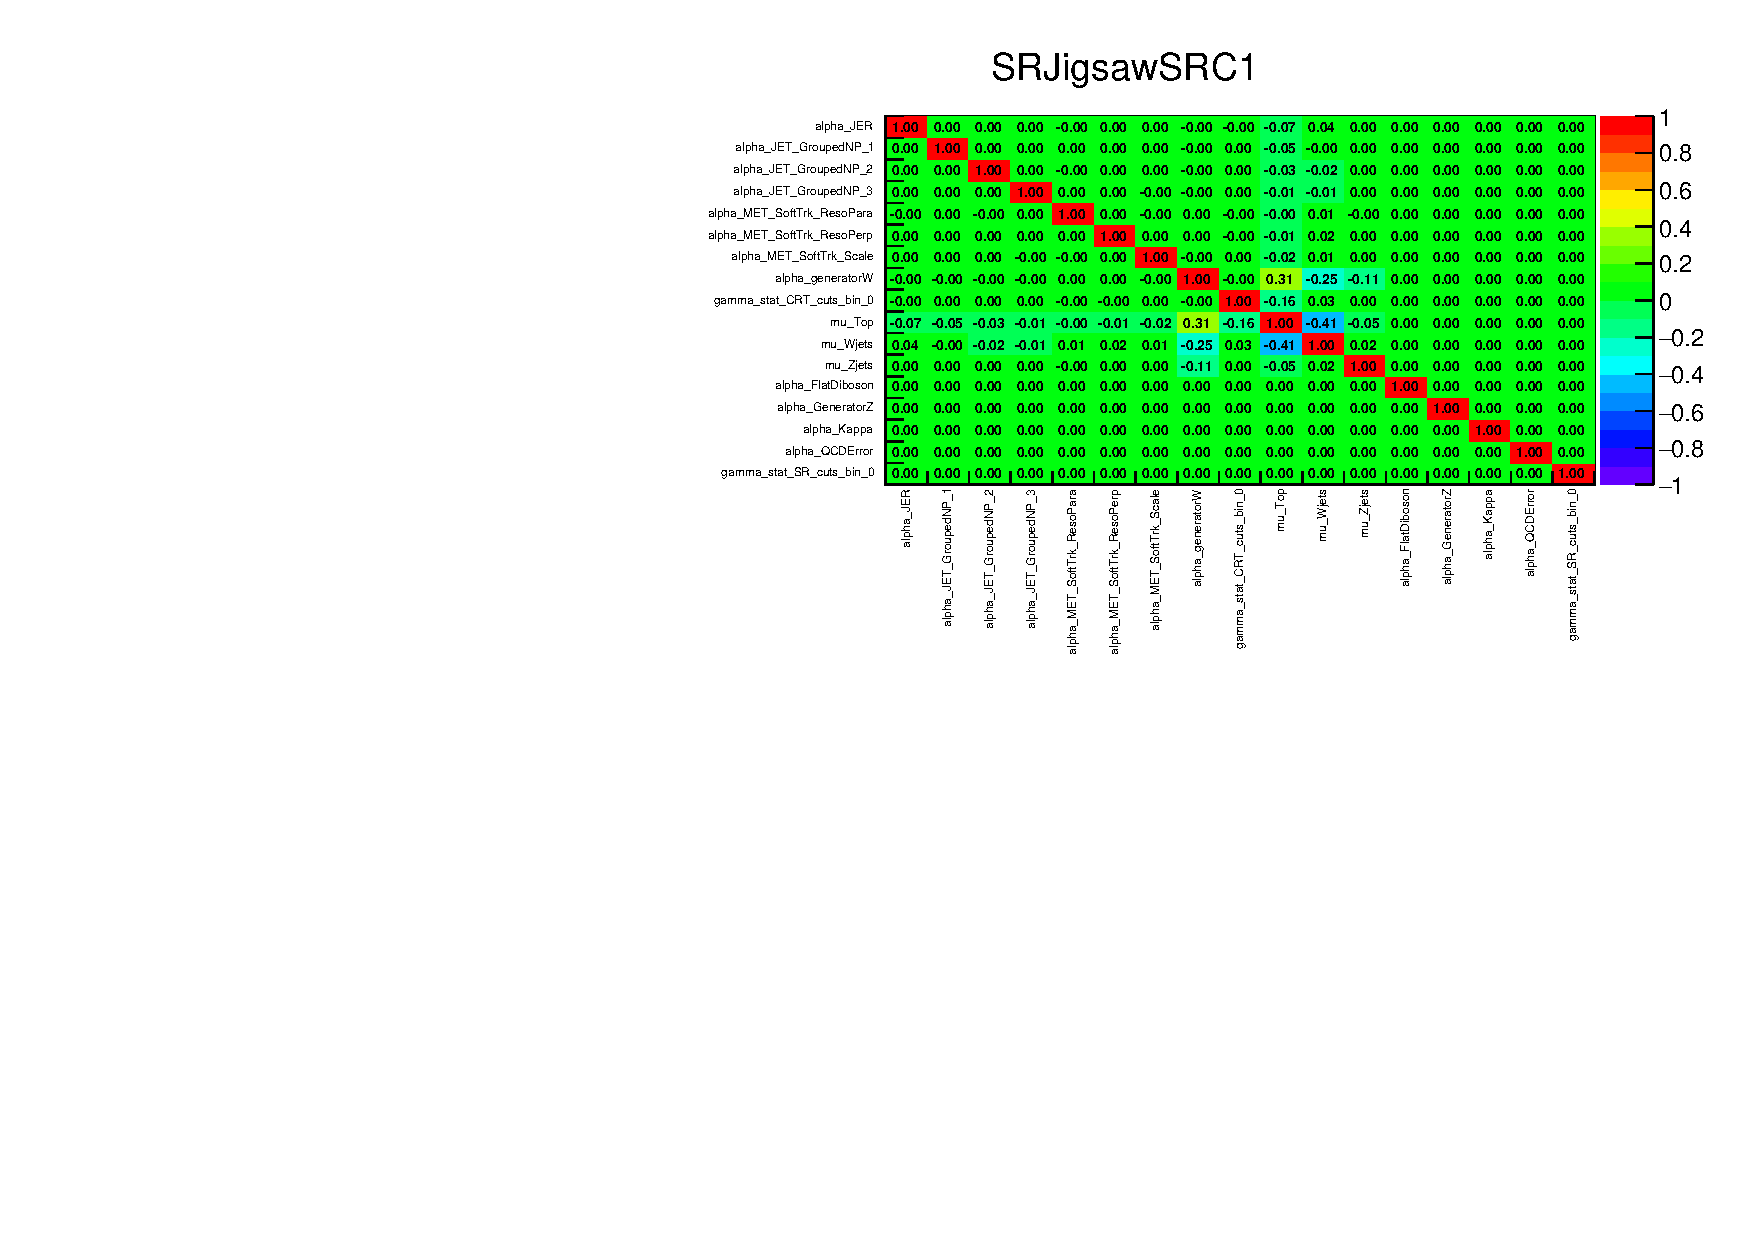
\includegraphics[width=.9\linewidth]{ATLAS-CONF-2016-078_INT/HistFitter/PullPlots/29_07_16/corr_SRJigsawSRC1}
% 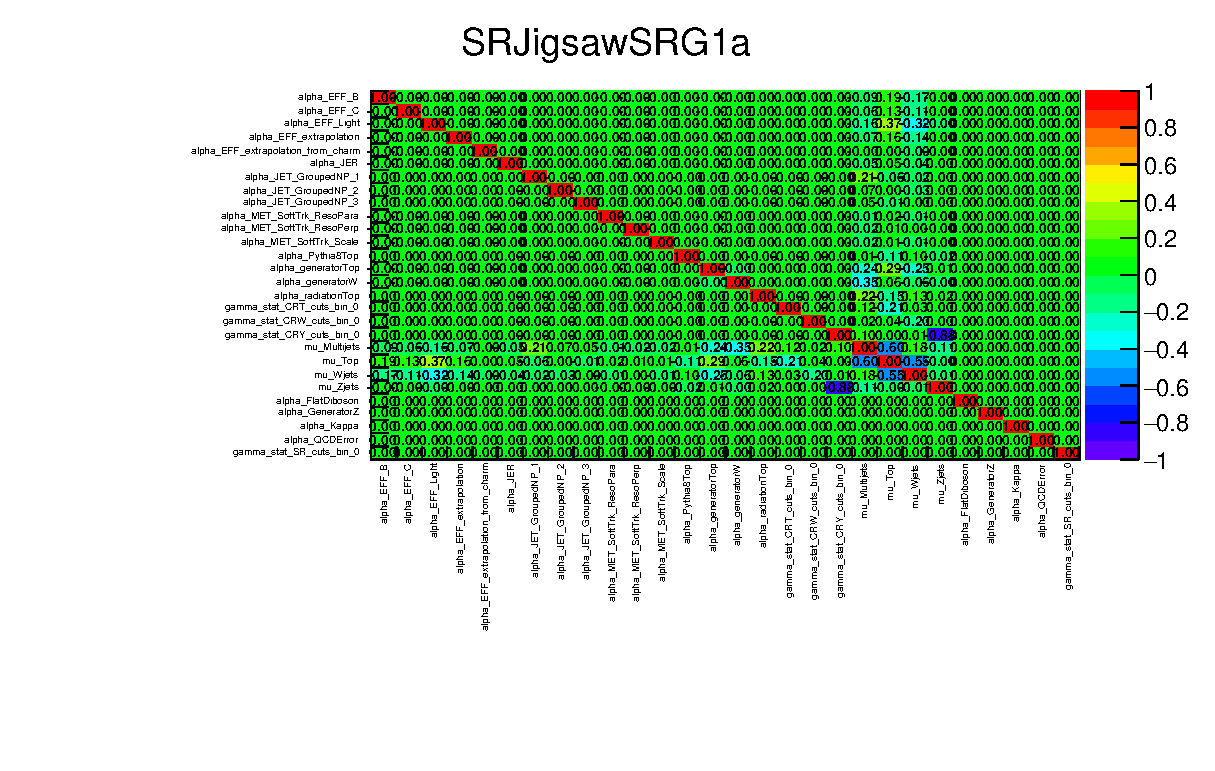
\includegraphics[width=.9\linewidth]{ATLAS-CONF-2016-078_INT/HistFitter/PullPlots/29_07_16/corr_SRJigsawSRG1a}
% 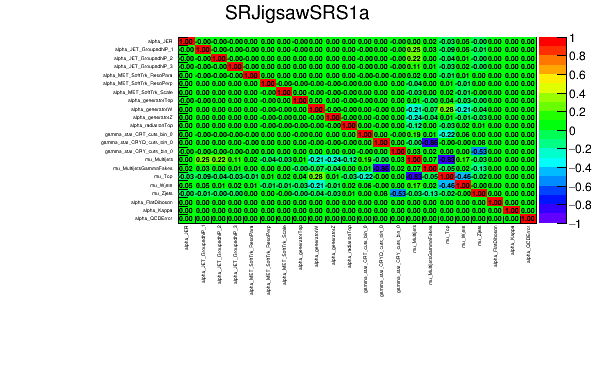
\includegraphics[width=.9\linewidth]{ATLAS-CONF-2016-078_INT/HistFitter/PullPlots/29_07_16/corr_SRJigsawSRS1a}
% \end{figure}

%% This table is automatically generated from individual tables per signal region
%% you can update it via the script: ./makeAllSystTableInOne.py

\begin{table}[tbp]
%\small
\scriptsize
\begin{center}
%\begin{sidewaystable}
%\scriptsize
%\begin{center}
%\setlength{\tabcolsep}{0.0pc}
\begin{tabular}{|lrrrrrr|}
\hline
Channel  &  \textbf{ S1a } & \textbf{ S1b } & \textbf{ S2a } & \textbf{ S2b } & \textbf{ S3a } & \textbf{ S3b }  \\ \hline
Total bkg  &  $334$  &  $233$  &  $96$  &  $75$  &  $56$  &  $37$ \\
Total bkg unc.  &  $\pm 35$  [$10\%$]  &  $\pm 25$  [$11\%$]  &  $\pm 10$  [$10\%$]  &  $\pm 8$  [$11\%$]  &  $\pm 6$  [$11\%$]  &  $\pm 4$  [$11\%$] \\
\hline
MC statistics  &   --    &  $\pm 2.6$ [$1\%$]  &  $\pm 1.5$ [$2\%$]  &  $\pm 1.3$ [$2\%$]  &  $\pm 1.0$ [$2\%$]  &  $\pm 0.7$ [$2\%$] \\
$\Delta\mu_{Z,\mathrm{+jets}}$    &  $\pm 20$ [$6\%$]  &  $\pm 14$ [$6\%$]  &  $\pm 4$ [$4\%$]  &  $\pm 2.9$ [$4\%$]  &  $\pm 2.2$ [$4\%$]  &  $\pm 1.5$ [$4\%$] \\
$\Delta\mu_{W,\mathrm{+jets}}$    &  $\pm 10$ [$3\%$]  &  $\pm 7$ [$3\%$]  &  $\pm 3.1$ [$3\%$]  &  $\pm 2.3$ [$3\%$]  &  $\pm 1.6$ [$3\%$]  &  $\pm 1.1$ [$3\%$] \\
$\Delta\mu_{  \mathrm{ Top}}$       &  $\pm 6$ [$2\%$]  &  $\pm 4$ [$2\%$]  &  $\pm 1.5$ [$2\%$]  &  $\pm 1.1$ [$1\%$]  &  $\pm 0.9$ [$2\%$]  &  $\pm 0.6$ [$2\%$] \\
$\Delta\mu_{  \mathrm{ Multijet}}$  &  $\pm 0.09$ [$0\%$]  &  $\pm 0.05$ [$0\%$]  &  $\pm 0.02$ [$0\%$]  &   --    &   --    &   --   \\
CR$\gamma$ corr. factor  &  $\pm 12$ [$4\%$]  &  $\pm 8$ [$3\%$]  &  $\pm 4$ [$4\%$]  &  $\pm 2.9$ [$4\%$]  &  $\pm 2.2$ [$4\%$]  &  $\pm 1.4$ [$4\%$] \\
Theory Z  &  $\pm 23$ [$7\%$]  &  $\pm 16$ [$7\%$]  &  $\pm 7$ [$7\%$]  &  $\pm 6$ [$8\%$]  &  $\pm 4$ [$7\%$]  &  $\pm 2.8$ [$8\%$] \\
Theory W  &  $\pm 4$ [$1\%$]  &  $\pm 5$ [$2\%$]  &  $\pm 0.4$ [$0\%$]  &  $\pm 0.11$ [$0\%$]  &  $\pm 1.5$ [$3\%$]  &  $\pm 1.2$ [$3\%$] \\
Theory Top   &  $\pm 4$ [$1\%$]  &  $\pm 2.7$ [$1\%$]  &  $\pm 0.8$ [$1\%$]  &  $\pm 0.7$ [$1\%$]  &  $\pm 0.6$ [$1\%$]  &  $\pm 0.4$ [$1\%$] \\
Theory Diboson  &  $\pm 9$ [$3\%$]  &  $\pm 6$ [$3\%$]  &  $\pm 2.8$ [$3\%$]  &  $\pm 2.6$ [$3\%$]  &  $\pm 2.1$ [$4\%$]  &  $\pm 1.4$ [$4\%$] \\
Jet/MET   &  $\pm 3.3$ [$1\%$]  &  $\pm 1.5$ [$1\%$]  &  $\pm 0.6$ [$1\%$]  &  $\pm 0.6$ [$1\%$]  &  $\pm 1.2$ [$2\%$]  &  $\pm 1.0$ [$3\%$] \\
Multijet method  &  $\pm 0.7$ [$0\%$]  &  $\pm 0.4$ [$0\%$]  &  $\pm 0.08$ [$0\%$]  &   --    &   --    &   --   \\
\hline
\end{tabular}

\begin{tabular}{|lrrrrrr|}
\hline
Channel  &  \textbf{ G1a } & \textbf{ G1b } & \textbf{ G2a } & \textbf{ G2b } & \textbf{ G3a } & \textbf{ G3b }  \\ \hline
Total bkg  &  $40$  &  $18.8$  &  $27.8$  &  $8.5$  &  $5.8$  &  $1.7$ \\
Total bkg unc.  &  $\pm 4$  [$10\%$]  &  $\pm 2.5$  [$13\%$]  &  $\pm 3.4$  [$12\%$]  &  $\pm 1.4$  [$16\%$]  &  $\pm 1.1$  [$19\%$]  &  $\pm 0.4$  [$24\%$] \\
\hline
MC statistics  &  $\pm 1.6$ [$4\%$]  &  $\pm 1.0$ [$5\%$]  &  $\pm 1.2$ [$4\%$]  &  $\pm 0.6$ [$7\%$]  &  $\pm 0.4$ [$7\%$]  &  $\pm 0.23$ [$14\%$] \\
$\Delta\mu_{Z,\mathrm{+jets}}$  &  $\pm 1.5$ [$4\%$]  &  $\pm 0.7$ [$4\%$]  &  $\pm 1.6$ [$6\%$]  &  $\pm 0.5$ [$6\%$]  &  $\pm 0.4$ [$7\%$]  &  $\pm 0.1$ [$6\%$] \\
$\Delta\mu_{W,\mathrm{+jets}}$  &  $\pm 0.9$ [$2\%$]  &  $\pm 0.4$ [$2\%$]  &  $\pm 1.2$ [$4\%$]  &  $\pm 0.31$ [$4\%$]  &  $\pm 0.28$ [$5\%$]  &  $\pm 0.1$ [$6\%$] \\
$\Delta\mu_{\mathrm{ Top}}$  &  $\pm 0.8$ [$2\%$]  &  $\pm 0.33$ [$2\%$]  &  $\pm 0.9$ [$3\%$]  &  $\pm 0.23$ [$3\%$]  &  $\pm 0.07$ [$1\%$]  &  $\pm 0.1$ [$6\%$] \\
$\Delta\mu_{\mathrm{ Multijet}}$  &  $\pm 0.1$ [$0\%$]  &  --  &  $\pm 0.03$ [$0\%$]  &  $\pm 0.02$ [$0\%$]  &   --    &   --   \\
CR$\gamma$ corr. factor  &  $\pm 1.2$ [$3\%$]  &  $\pm 0.6$ [$3\%$]  &  $\pm 0.8$ [$3\%$]  &  $\pm 0.26$ [$3\%$]  &  $\pm 0.19$ [$3\%$]  &  $\pm 0.05$ [$3\%$] \\
Theory Z  &  $\pm 2.3$ [$6\%$]  &  $\pm 1.1$ [$6\%$]  &  $\pm 1.6$ [$6\%$]  &  $\pm 0.5$ [$6\%$]  &  $\pm 0.4$ [$7\%$]  &  $\pm 0.1$ [$6\%$] \\
Theory W  &  $\pm 1.1$ [$3\%$]  &  $\pm 1.3$ [$7\%$]  &  $\pm 0.3$ [$1\%$]  &  $\pm 0.7$ [$8\%$]  &  $\pm 0.6$ [$10\%$]  &  $\pm 0.16$ [$9\%$] \\
Theory Top   &  $\pm 1.2$ [$3\%$]  &  $\pm 0.7$ [$4\%$]  &  $\pm 1.0$ [$4\%$]  &  $\pm 0.4$ [$5\%$]  &  $\pm 0.4$ [$7\%$]  &  $\pm 0.26$ [$15\%$] \\
Theory Diboson  &  $\pm 1.3$ [$3\%$]  &  $\pm 0.8$ [$4\%$]  &  $\pm 1.5$ [$5\%$]  &  $\pm 0.6$ [$7\%$]  &  $\pm 0.31$ [$5\%$]  &  $\pm 0.13$ [$8\%$] \\
Jet/MET   &  $\pm 1.0$ [$3\%$]  &  $\pm 0.6$ [$3\%$]  &  $\pm 0.4$ [$1\%$]  &  $\pm 0.17$ [$2\%$]  &  $\pm 0.22$ [$4\%$]  &  $\pm 0.05$ [$3\%$] \\
Multijet method  &  $\pm 0.24$ [$1\%$]  &  $\pm 0.12$ [$1\%$]  &  $\pm 0.5$ [$2\%$]  &  $\pm 0.4$ [$5\%$]  &   --    &   --   \\
\hline
\end{tabular}

\begin{tabular}{|lrrrrr|}
\hline
Channel                           & \textbf{ C1 }   & \textbf{ C2 }  & \textbf{ C3 }  & \textbf{ C4 }   & \textbf{ C5 }   \\ \hline
Total bkg                         & $14.5$              & $59$               & $110$              & $10.5$              & $7.3$               \\
Total bkg unc.                    & $\pm 2.2$  [$15\%$] & $\pm 6$  [$10\%$]  & $\pm 11$  [$10\%$] & $\pm 1.5$  [$14\%$] & $\pm 1.4$  [$19\%$] \\
\hline
MC statistics                     & $\pm 0.7$ [$5\%$]   & $\pm 1.7$ [$3\%$]  & $\pm 2.4$ [$2\%$]  & $\pm 0.6$ [$6\%$]   & $\pm 0.6$ [$8\%$]   \\
$\Delta\mu_{Z,\mathrm{+jets}}$    & $\pm 0.5$ [$3\%$]   & $\pm 1.9$ [$3\%$]  & $\pm 2.5$ [$2\%$]  & $\pm 0.31$ [$3\%$]  & $\pm 0.13$ [$2\%$]  \\
$\Delta\mu_{W,\mathrm{+jets}}$    & $\pm 0.4$ [$3\%$]   & $\pm 1.7$ [$3\%$]  & $\pm 5$ [$5\%$]    & $\pm 0.4$ [$4\%$]   & $\pm 0.25$ [$3\%$]  \\
$\Delta\mu_{\mathrm{ Top}}$       & $\pm 0.33$ [$2\%$]  & $\pm 1.3$ [$2\%$]  & $\pm 4$ [$4\%$]    & $\pm 0.31$ [$3\%$]  & $\pm 0.4$ [$5\%$]   \\
$\Delta\mu_{\mathrm{ Multijet}}m$ & --                  & $\pm 0.1$ [$0\%$]  & $\pm 0.06$ [$0\%$] & --                  & $\pm 0.1$ [$1\%$]   \\
CR$\gamma$ corr. factor $\kappa$  & $\pm 0.5$ [$3\%$]   & $\pm 1.8$ [$3\%$]  & $\pm 2.3$ [$2\%$]  & $\pm 0.29$ [$3\%$]  & $\pm 0.13$ [$2\%$]  \\
Theory Z                          & $\pm 0.8$ [$6\%$]   & $\pm 3.5$ [$6\%$]  & $\pm 4$ [$4\%$]    & $\pm 0.6$ [$6\%$]   & $\pm 0.24$ [$3\%$]  \\
Theory W                          & $\pm 1.3$ [$9\%$]   & $\pm 0.03$ [$0\%$] & $\pm 2.0$ [$2\%$]  & $\pm 1.0$ [$10\%$]  & $\pm 0.13$ [$2\%$]  \\
Theory Top                        & $\pm 0.5$ [$3\%$]   & $\pm 1.3$ [$2\%$]  & $\pm 3.2$ [$3\%$]  & $\pm 0.6$ [$6\%$]   & $\pm 0.9$ [$12\%$]  \\
Theory Diboson                    & $\pm 1.0$ [$7\%$]   & $\pm 4$ [$7\%$]    & $\pm 6$ [$5\%$]    & $\pm 0.27$ [$3\%$]  & $\pm 0.4$ [$5\%$]   \\
Jet/MET                           & $\pm 0.5$ [$3\%$]   & $\pm 1.5$ [$3\%$]  & $\pm 3.1$ [$3\%$]  & $\pm 0.24$ [$2\%$]  & $\pm 0.5$ [$7\%$]   \\
Multijet method                   & $\pm 0.09$ [$1\%$]  & $\pm 0.4$ [$1\%$]  & $\pm 2.1$ [$2\%$]  & --                  & $\pm 0.18$ [$2\%$]  \\
\hline
\end{tabular}

%\end{tabular*}
\end{center}
\caption{
Breakdown of the dominant systematic uncertainties in the background estimates.
The individual uncertainties can be correlated, and do not necessarily add in quadrature.
$\Delta_{\mu}$ uncertainties result from control region statistical uncertainties and the systematic uncertainties in the appropriate control region.
In brackets, uncertainties are given relative to the expected total background yield, also presented in the Table. Empty cells (indicated by a `-') correspond to uncertainties $<$0.1\%. \label{tab:BreakdownSysSRCompressed_RJR}}
%\end{sidewaystable}
\end{table}


\section{Model-Independent Limits and Model-dependent Exclusions}

In \Cref{tab:BreakdownSysSRCompressed_RJR}, we show the one-sided $p$-value ($p_0$) and the equivalent statistical significance Z for each signal region:
\begin{align}
Z = \frac{N_{\mathrm{obs}} - N_{\mathrm{pred}}}{\sigma_{\mathrm{tot}}}
\end{align}
We calculate this using the fitted simulation mean compared with the observed event counts in each region.
There is no significant excess in any of the signal region; the largest excess is in SRG3b with $Z_{\text{SRG3b}} = 1.55$.
This information is summarized in \Cref{fig:sr_summary}.
We thus set model-independent and model-dependent limits.

\subsection{Model-Independent Limits}

As no significant excess is observed in any of the signal regions of this analysis after estimating the background using the background-only fit, we set limits on the model-independent and model-dependent cross sections.
We use the model-independent and model-dependent fit setups.

The model-independent limits are shown in \Cref{tab:BreakdownSysSRCompressed_RJR}.
We present the upper limits on the cross-section for new physics which enters each SR.
%These model-independent limits have no limitations based on the expected signal models.
The observed and expected limits \sobs and \sexp are reported for the potential contribution from new physics in each region.
Including the acceptance $\epsilon$, the model-independent limits in most signal regions are of $\order 1-2$ fb.
One should note that the (b) version of each signal region has a strictly tighter cut on the primary scale variable, and thus provides a stronger limit when we observe no excess.

\subsection{Model-Dependent Limits and Exclusions}

We derive exclusion limits for the simplified models.
These are models with pair-production of squark pairs with inaccessible gluinos, and gluino pairs with inaccessible squarks.
They correspond directly to the Feynman diagrams shown previously.
The free parameters of these simplified models are the relevant sparticle mass and the mass of the LSP \lsp.
We set limits the plane of these free parameters.

The exclusion limits are shown in \Cref{fig:sensitivitytext}.
%The gray text at the point of each simplified model with masses $(m_{\mathrm{sparticle}}, m_{\lsp})$
The gray text indicates the signal region providing the best sensitivity at that $(m_{\mathrm{sparticle}}, m_{\lsp})$ point, as measured by the background-only fit.
For each simplified signal model, we run the model-dependent fit, where the signal model signal strength $\mu_{\mathrm{sig}}$ is included as an additional free parameter.
The signal sample can also contribute to the control regions due to signal contamination.
This produces a CL$_s$ $p-$value for each signal model in the plane, and we can find those with $p = 0.05$ to set a 95\% exclusion limit.
For comparison, the limits from the 2015 dataset and the 2012 dataset are also shown.
%The simultaneous fit in the control and signal region produces a set of normalization parameters $\mu$ for each Standard Model background as well as the signal strength $\mu_{\mathrm{sig}}$ for the particular signal model of interest.

In the squark-\lsp~ exclusion plane in \Cref{fig:exclusion_sq}, the limits are far extended compared to the 2015 dataset.
The expected and observed exclusions are similar, which reflects the compatability of the expected Standard Model event counts and observed event counts in the squark signal regions.
A squark with mass of 1350 \GeV~ or less is excluded by the analysis in direct decays to a quark and massless LSP.
In the compressed spectra, we extended limits significantly over the 2015 result in the region of 600-700 \GeV~ in squark mass with an LSP of 450 \GeV~ to 600 \GeV~.
Directly along the kinematically-forbidden diagonal, the shape of the exclusions are artificially affected by the interpolation between the signal models considered.
This artificial effect can be resolved by the simulation of additional signal models to fill in the space.
The limits in the intermediate with an LSP of \order 450-500 \GeV~ are not significantly extended beyond the previous dataset.
Each signal region designed to provide sensitivity to the squark pair-production model (all SRS regions and SRC1-4) excludes at least one point in the grid.
This indicating each signal region provides additional sensitivity to squark phenomena, or more explicitly, we would exclude a smaller region of the squark pair-production simplified model space with fewer signal regions.

Curiously, a gluino region, SRG2a, is chosen as the optimal signal region in the squark-\lsp~ plane, when the squark mass is \order 700 \GeV.
Generally, the squark regions are looser than the gluino regions, as seen in their overall event yields.
One could see this as an indication that the next iteration of the analysis should have an additional tight squark region targeting this point in the plane.
Another possibility is this region also benefits from the ISR-assisted compressed region strategy.
As the gluino regions require four jets due to the imposition of the gluino decay tree, these could be capturing events where a two jet ISR system recoils off the disquark system.

In the gluino-\lsp~ exclusion plane shown in \Cref{fig:exclusion_gl}, the limits on gluino masses in the simplified model where gluinos decay to two jets and an \lsp~ significantly extend the limits from the 2015 dataset.
Throughout most of the plane, the expected limit is significantly stronger than the observed limit; for example, the gluino mass limit is more than 50 \GeV~ stronger in the case of a massless \lsp~.
A significant portion of phase space is covered by SRG3a and SRG3b.
These regions saw a statistical fluctuation upward, seen in the signal region pulls \Cref{fig:sr_summary}.
The weaker observed limits are simply a result of this fluctuation.
We emphasize that every gluino signal region is the best choice at some point in this plane.
This indicates each signal region provides additional sensitivity to some portion of the phase space of simplified models, and thus lead to stronger exclusions.

\begin{figure}[tbp]
\begin{center}
\subfloat[]{\label{fig:exclusion_sq}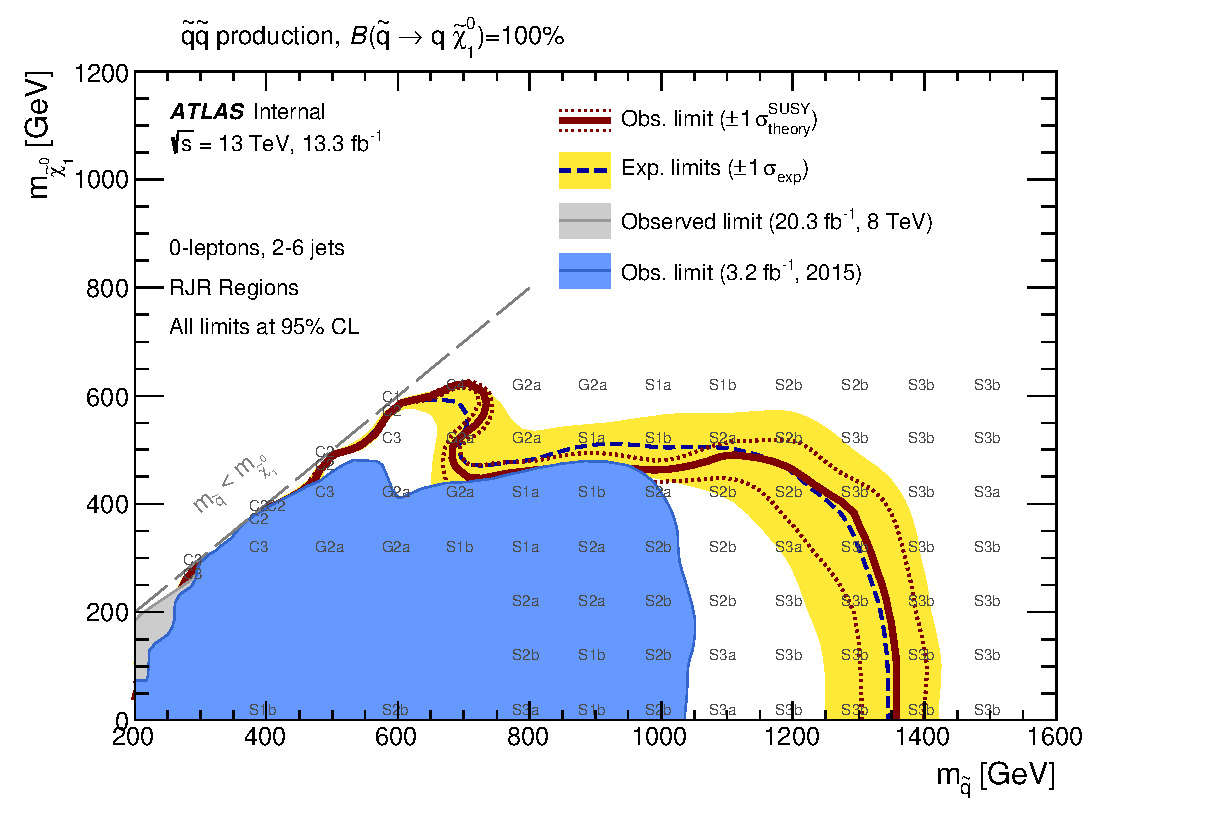
\includegraphics[width=0.9\textwidth]{figures/ATLAS-CONF-2016-078_INT/Sensitivity/RJR/atlasCLs_SS_direct_showSR}}\\
\subfloat[]{\label{fig:exclusion_gl}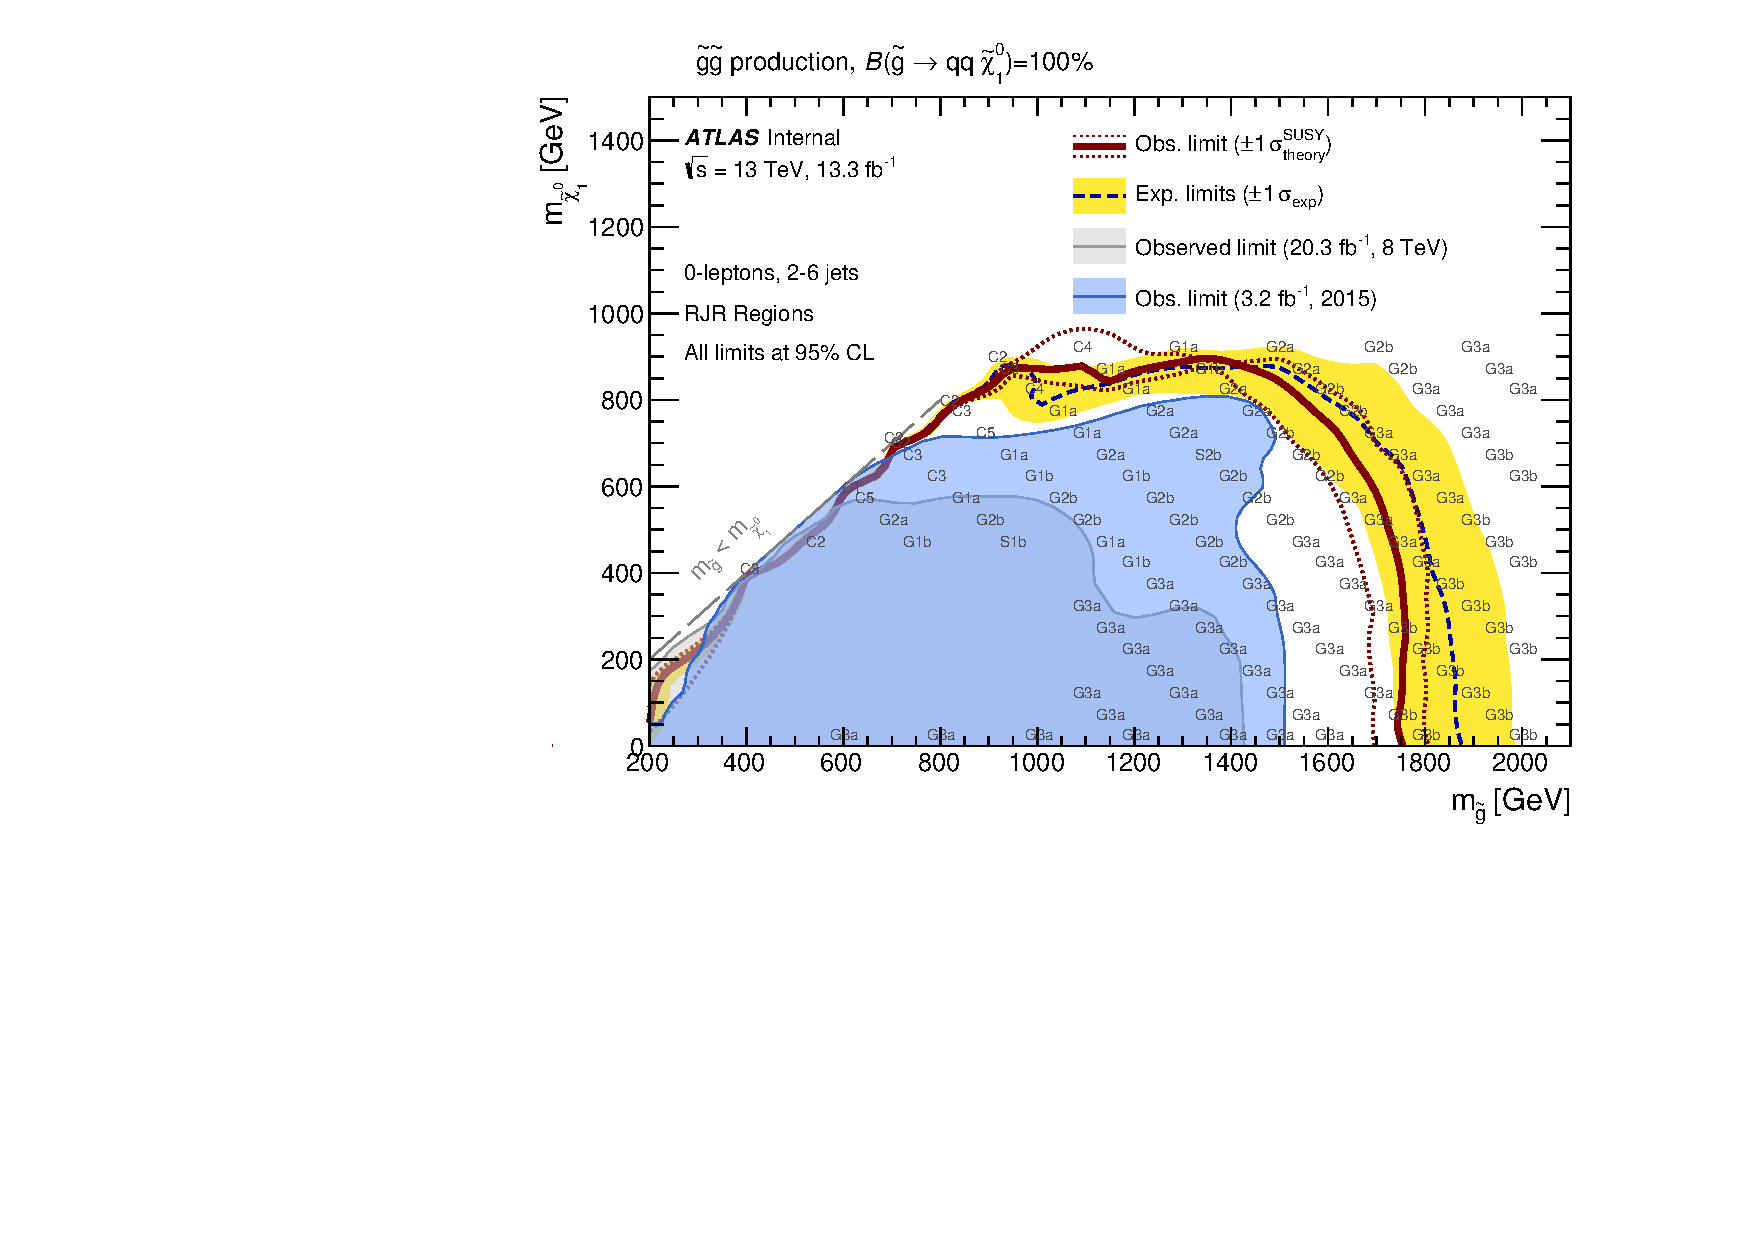
\includegraphics[width=0.9\textwidth]{figures/ATLAS-CONF-2016-078_INT/Sensitivity/RJR/atlasCLs_GG_direct_showSR}}
\end{center}
\caption{Exclusion limits for direct production of (a) light-flavour squark pairs with decoupled gluinos and (b) gluino pairs with decoupled squarks.
Exclusion limits are obtained from the signal region with the best expected sensitivity at each point.
The blue dashed lines show the expected limits at 95\% CL, with the yellow bands indicating the $1\sigma$ exclusions.
Observed limits are indicated by maroon curves where the solid contour represents the nominal limit and the dashed countours indicate the $1\sigma$ exclusions.
}
\label{fig:sensitivitytext}
\end{figure}
